%%%%%%%%%%%%%%%%%%%%%%%%%%%%%%%%%%%%%%%%%%%%%%%%%%%%%%%%%%%%
%%%%%%%%%%%%%%%%%%%%%%%%%%%%%%%%%%%%%%%%%%%%%%%%%%%%%%%%%%%%
%%%%%%%%%%%%%%%%%%%%%%%%%%%%%%%%%%%%%%%%%%%%%%%%%%%%%%%%%%%%
\section{The Dune Workflow for Simulations with CAD-Models}\label{Sec:Workflow}
%%%%%%%%%%%%%%%%%%%%%%%%%%%%%%%%%%%%%%%%%%%%%%%%%%%%%%%%%%%%
%%%%%%%%%%%%%%%%%%%%%%%%%%%%%%%%%%%%%%%%%%%%%%%%%%%%%%%%%%%%
%%%%%%%%%%%%%%%%%%%%%%%%%%%%%%%%%%%%%%%%%%%%%%%%%%%%%%%%%%%%

\begin{frame}
  \frametitle<presentation>{Abstraction}
  \begin{itemize}
    \item Real world problems have complex computational domains.
      require abstraction.
    \item Abstractions for function spaces.
    \item Abstractions for PDE discretizations.
  \end{itemize}
\end{frame}

\subsection{Overview}
% Bilder
% Tool Chain

%\begin{frame}
%\frametitle{Problem and Weak Formulation}
%Consider the following model problem:
%\begin{subequations} \label{Eq:Example01}
%\begin{align*}
%-\Delta u + a u &= f &&\text{in $\Omega\subset\mathbb{R}^d$ (open, connected)},\\
%\nabla u \cdot n &= 0 &&\text{on $\partial\Omega$}.
%\end{align*}
%\end{subequations}
%\medskip
%Weak formulation. Set $U = H^1(\Omega)$.
%\begin{equation*}
%u\in U \quad : \quad \underbrace{\int_\Omega \nabla u \cdot \nabla v +
%a u v - f v \,dx}_{r(u,v)} = 0 \qquad \forall v\in U.
%\end{equation*}
%Has unique solution for $a(x)\geq a_0>0$.
%
%We call $r(u,v)$ residual form.
%
%Other boundary conditions are treated later.
%\end{frame}
%
%\begin{frame}
%\frametitle{Conforming Finite Element Method}
%Needs conforming triangulation $E_h^0 = \{e_o,\ldots,e_{N_h^0-1} \}$ of $\Omega$.
%
%Define the conforming finite element space
%\begin{equation*}
%U_h^k = \left\{  u\in C^0(\overline{\Omega}) \ : \ u|_{\Omega_e} \in P_{k_e} \forall e\in E_h^0\right\} \subset H^1(\Omega).
%\end{equation*}
%\begin{itemize}
%\item $\Omega_e$: domain of element $e\in E_h^0$.
%\item $P_k$: Polynomials of degree $k$.
%\item $k_e$: Polynomial degree on element $e$.
%\end{itemize}
%Discrete problem then reads:
%\begin{equation*}
%u_h \in U_h^k \quad : \quad r(u_h,v) = 0 \qquad \forall v \in U_h^k.
%\end{equation*}
%\end{frame}
%
%\begin{frame}
%\frametitle{Affine Finite Element Spaces}
%Construct functions in $U_h^k$ from local basis on reference elements:
%\begin{equation*}
%U_h^k\ni u_h(x) = \sum_{e\in E_h^0} \sum_{l=0}^{n(e)-1} (\mathbf{u})_{g(e,l)}
%\, \hat{\phi}_{e,l}(\mu_e^{-1}(x)) \, \chi_e(x).
%\end{equation*}
%\begin{itemize}
%\item $n(e)$: Number of basis functions on element $e\in E_h^0$.
%\item $\hat\Omega_e$: Reference element of element $e\in E_h^0$.
%\item $\mu_e : \hat\Omega_e \to \Omega_e$: Element transformation.
%\item $\hat\phi_{e,l} : \hat\Omega_e \to \mathbb{R}$: Local basis function.
%\item $\mathcal{I}_{U_h^k} = \{0,\ldots,N_{U_h^k}-1\}$: Global index set.
%\item $g : E_h^0 \times \mathbb{N}_0 \to \mathcal{I}_{U_h^k}$: Local to global index map.
%\item $\mathbf{u} \in \mathbf{U} = \mathbb{R}^{\mathcal{I}_{U_h^k}}$: Global vector of degrees of freedom.
%\item $\chi_e$: Characteristic function of element $e$.
%\end{itemize}
%Note: We might have a different set of basis functions on each element.
%\end{frame}
%
%\begin{frame}
%\frametitle{Global Basis; Finite Element Isomorphism}
%For $j\in \mathcal{I}_{U_h^k}$ set $L(j) = \{ (e,l) \, : \, g(e,l) = j\}$ (all local degrees
%of freedom associated with global degree of freedom $j$.
%
%Global basis:
%\begin{equation*}
%\Phi_{U_h^k} = \left\{ \phi_j(x) = \sum_{(e,l)\in L(j)} \hat{\phi}_{e,l}(\mu_e^{-1}(x)) \, \chi_e(x)
%\, : \, j \in \mathcal{I}_{U_h^k} \right\}.
%\end{equation*}
%
%Finite Element Isomorphism:
%\begin{align*}
%\text{FE}_{\Phi_{U_h^k}} : \mathbf{U} &\to U_h^k, &
%\text{FE}_{\Phi_{U_h^k}}(\mathbf{u}) &= \sum_{j\in \mathcal{I}_{U_h^k}} (\mathbf{u})_j \phi_j.
%\end{align*}
%\end{frame}
%
%\begin{frame}
%\frametitle{Algebraic Problem}
%Using the basis the discrete problem can be written equivalently as a (in general nonlinear) algebraic problem:
%\begin{align*}
%&&& u_h \in U_h^k \quad : \quad r(u_h,v) = 0 && \forall v \in U_h^k,\\
%&\Leftrightarrow && \mathbf{u}\in\mathbf{U} \quad : \quad
%r\left(\text{FE}_{\Phi_{U_h^k}}(\mathbf{u}),\phi_i\right) = 0 &&
%i\in\mathcal{I}_{U_h^k}, \\
%&\Leftrightarrow && \mathbf{u}\in\mathbf{U} \quad : \quad
%\mathcal{R}(\mathbf{u}) = \mathbf{0}.
%\end{align*}
%where
%\begin{align*}
%\mathcal{R} &: \mathbf{U} \to \mathbf{U}, &
%\left(\mathcal{R}(\mathbf{u}) \right)_i :=  r\left(\text{FE}_{\Phi_{U_h^k}}(\mathbf{u}),\phi_i\right) .
%\end{align*}
%
%For linear PDEs $\mathcal{R}$ is affine linear: $\mathcal{R}(\mathbf{u}) = \mathbf{A} \mathbf{u} - \mathbf{b}$.
%\end{frame}
%
%\begin{frame}
%\frametitle{Residual Assembly}
%\begin{equation*}
%\begin{split}
%&(\mathcal{R}(\mathbf{u}) )_i  = r\left(\text{FE}(\mathbf{u}),\phi_i\right)
%= \sum_{e\in E_h^0} \int_{\Omega_e} \nabla \text{FE}(\mathbf{u}) \cdot \nabla\phi_i
%+ a \, \text{FE}_{\Phi_{U_h^k}}(\mathbf{u}) \phi_i - f \phi_i \,dx\\
%&= \sum_{e\in E_h^0} \int_{\Omega_e}
%\left[ \sum_{l=0}^{n(e)-1} (\mathbf{u})_{g(e,l)} \nabla_x \hat\phi_{e,l}(\mu_e^{-1}(x))\right]
%\cdot \nabla_x \underbrace{\hat\phi_{e,m}}_{g(e,m)=i}(\mu_e^{-1}(x))\\
%& + a \, \left[ \sum_{l=0}^{n(e)-1} (\mathbf{u})_{g(e,l)} \hat\phi_{e,l}(\mu_e^{-1}(x)) \right] \hat\phi_{e,m}(\mu_e^{-1}(x))
%- f \hat\phi_{e,m}(\mu_e^{-1}(x)) \, dx\\
%&= \sum_{e\in E_h^0} \int_{\hat\Omega_e}
%\Biggl\{\left[ \sum_{l=0}^{n(e)-1} (\mathbf{u})_{g(e,l)} (\nabla \mu_e(\hat{x}))^{-T}\nabla_{\hat{x}} \hat\phi_{e,l}(\hat{x})\right]
%\cdot (\nabla \mu_e(\hat{x}))^{-T} \nabla_{\hat{x}} \hat\phi_{e,m}(\hat{x})\\
%& + a \, \left[ \sum_{l=0}^{n(e)-1} (\mathbf{u})_{g(e,l)} \hat\phi_{e,l}(\hat{x}) \right] \hat\phi_{e,m}(\hat{x})
%- f \hat\phi_{e,m}(\hat{x}) \Biggr\} \text{det} \nabla\mu_e(\hat{x}) \, d\hat{x} .
%\end{split}
%\end{equation*}
%\end{frame}
%
%\begin{frame}
%\frametitle{Local Operator}
%Define restriction to local degrees of freedom
%\begin{align*}
%\mathbf{U}_e &= \mathbb{R}^{n(e)}, &
%\mathbf{R}_e &: \mathbf{U} \to \mathbf{U}_e, &
%\left(\mathbf{U}_e(\mathbf{u})\right)_l &= (\mathbf{u})_{g(e,l)} \quad 0\leq l < n(e).
%\end{align*}
%Define \textit{local operator} $\bm{\alpha}^{\text{vol}}_{h,e} : \mathbf{U}_e \to \mathbf{U}_e$ (user part):
%\begin{equation*}
%\begin{split}
%&\bigl(\bm{\alpha}^{\text{vol}}_{h,e}({\color{cyan}\mathbf{u}})\bigr)_m  = \\
%&\sum_{e\in E_h^0} \int_{\hat\Omega_e}
%\Biggl\{\left[ \sum_{l=0}^{n(e)-1} ({\color{cyan}\mathbf{u}})_{l} {\color{purple}
%(\nabla \mu_e(\hat{x}))^{-T}} {\color{blue}\nabla_{\hat{x}} \hat\phi_{e,l}(\hat{x})} \right]
%\cdot {\color{purple}(\nabla \mu_e(\hat{x}))^{-T}} {\color{blue}\nabla_{\hat{x}} \hat\phi_{e,m}(\hat{x})}\\
%& + {\color{olive} a} \, \left[ \sum_{l=0}^{n(e)-1} ({\color{cyan}\mathbf{u}})_{l}
% {\color{blue}\hat\phi_{e,l}(\hat{x})} \right] {\color{blue}\hat\phi_{e,m}(\hat{x})}
%- {\color{olive} f} {\color{blue}\hat\phi_{e,m}(\hat{x})} \Biggr\} {\color{purple}\text{det} \nabla\mu_e(\hat{x})} \, d\hat{x} .
%\end{split}
%\end{equation*}
%Residual assembly is written generically:
%\begin{equation*}
%\mathcal{R}(\mathbf{u}) = \sum_{e\in E_h^0} \mathbf{R}_e^T \bm{\alpha}^{\text{vol}}_{h,e} (\mathbf{R}_e \mathbf{u})
%\end{equation*}
%\end{frame}
%
%
%\begin{frame}
%\frametitle{Solving the Algebraic System}
%Use damped Newton method.
%
%Given $\mathbf{u}^0\in\mathbf{U}$. Compute $\mathbf{r}^0 = \mathcal{R}(\mathbf{u}^0)$. Set $k=0$.
%
%Iterate until convergence:
%\begin{enumerate}
%\item Assemble Jacobian System $\mathbf{A}^k = \nabla\mathcal{R}(\mathbf{u}^k)$.
%\item Solve $\mathbf{A}^k \mathbf{z}^k = \mathbf{r}^k$ with some linear solver.
%\item Update $\mathbf{u}^{k+1} = \mathbf{u}^{k} - \sigma^k \mathbf{z}^{k+1}$. $\sigma\in(0,1]$.
%\item Compute new residual $\mathbf{r}^{k+1} = \mathcal{R}(\mathbf{u}^{k+1})$.
%\item Set $k = k +1$.
%\end{enumerate}
%
%We need methods to compute $\mathcal{R}(\mathbf{u})$ and $\nabla\mathcal{R}(\mathbf{u})$.
%\end{frame}
%
%\begin{frame}
%\frametitle{Jacobian}
%The Jacobian matrix is defined as
%\begin{equation*}
%(\mathbf{A}^k)_{i,j} = (\nabla\mathcal{R}(\mathbf{u}^k))_{i,j}
%= \frac{\partial (\mathcal{R})_i}{\partial (\mathbf{u})_j}(\mathbf{u}^k)
%= \sum_{e\in E_h^0} \frac{\partial (\bm{\alpha}_{h,e}^{\text{vol}})_m }{\partial (\mathbf{u})_l } (\mathbf{R}_e \mathbf{u}),
%\end{equation*}
%where $g(e,m)=l, g(e,l)=j$.
%
%Again, the Jacobian can be computed from local contributions:
%\begin{equation*}
%\mathbf{A}^k = \sum_{e\in E_h^0} \mathbf{R}_e^T \nabla\bm{\alpha}_{h,e}^{\text{vol}}(\mathbf{R}_e \mathbf{u}) \, \mathbf{R}_e.
%\end{equation*}
%
%The local Jacobians can be
%\begin{itemize}
%\item programmed explicitly by the user, or
%\item derived generically through numerical differentiation. This requires only coding
%of the local residual contributions $\bm{\alpha}_{h,e}^{\text{vol}}$.
%\end{itemize}
%\end{frame}
%
%
%\begin{frame}
%\frametitle{The Linear Case}
%is a special case of the nonlinear case \ldots
%\begin{enumerate}
%\item Given $\mathbf{u}^0\in\mathbf{U}$.
%\item Compute $\mathbf{r} = \mathcal{R}(\mathbf{u}^0)$.
%\item Assemble Jacobian System $\mathbf{A} = \nabla\mathcal{R}(\mathbf{u}^0)$.
%\item Solve $\mathbf{A} \mathbf{z} = \mathbf{r}$ with some linear solver.
%\item Update $\mathbf{u} = \mathbf{u}^{0} - \mathbf{z}$.
%\end{enumerate}
%\end{frame}

\subsection{The DUNE Gmsh-Reader Interface}
% install with opencascade
% Dune\dotsGmshReader

%\begin{frame}
%\frametitle{Example 1 Overview}
%The first example implements model problem \eqref{Eq:Example01}.
%
%It consists of the following files:
%\begin{itemize}
%\item \lstinline{example01.cc} -- the file to be compiled.
%\item \lstinline{example01_main.hh} -- main function. Instantiates a grid and runs the variants.
%\item \lstinline{example01a_Q1.hh} -- solve model problem \eqref{Eq:Example01} with $Q_1$ elements.
%\item \lstinline{example01a_Q2.hh} -- same with $Q_2$ elements.
%\item \lstinline{example01a_RT.hh} -- same with nonconforming rotated bilinear (``Rannacher-Turek'' element).
%\item \lstinline{example01a_operator.hh} -- local operator implementing $\bm{\alpha}_{h,e}^{\text{vol}}$.
%\item \lstinline{example01b_Q2.hh} -- solve nonlinear variant of the model problem \eqref{Eq:Example01} with $Q_2$ elements.
%\item \lstinline{example01b_operator.hh} -- the local operator for the nonlinear variant.
%\end{itemize}
%\end{frame}
%
%\begin{frame}<presentation>[fragile,allowframebreaks,allowdisplaybreaks]
%\frametitle<presentation>{Function \lstinline{main}}
%\framesubtitle<presentation>{File \texttt{examples/example01\_main.hh}}
%\lstinputlisting[basicstyle=\tiny,numbers=left,
%numberstyle=\tiny, numbersep=2pt]{../../examples/example01_main.hh}
%\end{frame}
%\mode<article>{
%For completeness we show the main function that just instantiates a \lstinline{YaspGrid} object
%and calls the variants.
%
%Main functions will not be shown in later examples.
%
%\begin{Lst}[File examples/example01\_main.hh] \mbox
%\nopagebreak
%\lstinputlisting[basicstyle=\scriptsize,numbers=left,
%numberstyle=\tiny, numbersep=2pt]{../../examples/example01_main.hh}
%\end{Lst}}
%
%
%\begin{frame}
%\frametitle{Driver for Solving Stationary Linear Problems}
%\framesubtitle{About \lstinline{example01a_Q1.hh}}
%\begin{enumerate}
%\item Define useful constants/types like dimension or basic numeric type.
%\item Make \textit{grid function space} which corresponds here to $U_h^k$. It requires
%\begin{itemize}
%\item a \textit{finite element map} defining a local basis on each element.
%\item a method to set up \textit{constraints} on the function space (empty here).
%\item a suitable vector backend.
%\end{itemize}
%\item Make \textit{grid operator space} computing $\mathcal{R}(\mathbf{u})$, $\nabla\mathcal{R}(\mathbf{u})$. It requires
%\begin{itemize}
%\item a local operator which provides $\bm{\alpha}_{h,e}^{\text{vol}}$.
%\item trial and test grid function spaces, possibly with constraints.
%\item a suitable matrix backend.
%\end{itemize}
%\item Select a linear solver backend (see vector/matrix backend).
%\item Solve the linear problem given with the selected solver backend.
%\begin{itemize}
%\item \textit{Vector container} is used to store degrees of freedom $\mathbf{u}\in\mathbf{U}$.
%\end{itemize}
%\item Output graphics files to visualize solution with ParaView.
%\begin{itemize}
%\item \textit{Discrete grid function} implements finite element isomorphism.
%\end{itemize}
%\end{enumerate}
%\end{frame}
%
%
%\begin{frame}<presentation>[fragile,allowframebreaks,allowdisplaybreaks]
%\frametitle<presentation>{Unconstrained Elliptic Problem with $Q_1$}
%\framesubtitle<presentation>{File \texttt{examples/example01a\_Q1.hh}}
%\lstinputlisting[basicstyle=\tiny,numbers=left,
%numberstyle=\tiny, numbersep=2pt]{../../examples/example01a_Q1.hh}
%\end{frame}
%\mode<article>{
%\begin{Lst}[File examples/example01a\_Q1.hh] \mbox
%\nopagebreak
%\lstinputlisting[basicstyle=\scriptsize,numbers=left,
%numberstyle=\tiny, numbersep=2pt]{../../examples/example01a_Q1.hh}
%\end{Lst}}
%
%
%\begin{frame}
%\frametitle{Local Operator}
%\begin{itemize}
%\item The local operator implements $\bm{\alpha}_{h,e}^{\text{vol}}$ (and more).
%\item Class template \lstinline{GridOperatorSpace} builds on a local operator and
%provides $\mathcal{R}(\mathbf{u})$, $\nabla\mathcal{R}(\mathbf{u})$ \textit{generically}.
%\item Works for many different discretizations (see below).
%\item Works as well for systems of PDEs (see below).
%\end{itemize}
%\end{frame}
%
%\begin{frame}
%\frametitle{Local Operator Implementation}
%\framesubtitle{About \lstinline{example01a_operator.hh}}
%A local operator is a class providing the following:
%\begin{itemize}
%\item Flags controlling the sparsity pattern assembly.
%\item Method \lstinline{pattern_volume} assembling sparsity pattern (default provided).
%\item Flags controlling which terms to assemble.
%\item Method \lstinline{alpha_volume} computing $\bm{\alpha}_{h,e}^{\text{vol}}(\mathbf{u})$.
%\item Method \lstinline{jacobian_volume} computing $\nabla\bm{\alpha}_{h,e}^{\text{vol}}(\mathbf{u})$.
%This method can be provided generically through numerical differentiation.
%\item Method \lstinline{jacobian_apply_volume} computing $\nabla\bm{\alpha}_{h,e}^{\text{vol}}(\mathbf{u})\mathbf{u}$.
%This method can be provided generically through numerical differentiation.
%\item Possibly more methods (to be introduced later):
%\begin{itemize}
%\item \lstinline{alpha_boundary}, \lstinline{alpha_skeleton} -- boundary/interior face integrals.
%\item \lstinline{lambda_volume}, \lstinline{lambda_boundary} -- parts of the residual depending on the test function only (optional).
%\end{itemize}
%\end{itemize}
%\end{frame}
%
%\begin{frame}[fragile]
%\frametitle{\lstinline{alpha_volume} Method}
%The method \lstinline{alpha_volume} has the following signature:
%\begin{lstlisting}[basicstyle=\scriptsize]
%template<typename EG, typename LFSU, typename X,
%         typename LFSV, typename R>
%void alpha_volume (const EG& eg, const LFSU& lfsu, const X& x,
%                   const LFSV& lfsv, R& r) const;
%\end{lstlisting}
%Where the arguments are:
%\begin{itemize}
%\item \lstinline{eg} -- a codim 0 entity $e\in E_h^0$.
%\item \lstinline{lfsu} -- local basis $\hat\phi_{e,l}$ for trial space.
%\item \lstinline{x} -- local coefficients $(\mathbf{u})_l$.
%\item \lstinline{lfsv} -- local basis $\hat\psi_{e,l}$ for the test space
%\item \lstinline{r} -- local contribution to residual (the result).
%\end{itemize}
%\end{frame}
%
%
%\begin{frame}<presentation>[fragile,allowframebreaks,allowdisplaybreaks]
%\frametitle<presentation>{Local Operator for Unconstrained Elliptic Problem}
%\framesubtitle<presentation>{File \texttt{examples/example01a\_operator.hh}}
%\lstinputlisting[basicstyle=\tiny,numbers=left,
%numberstyle=\tiny, numbersep=2pt]{../../examples/example01a_operator.hh}
%\end{frame}
%\mode<article>{
%\begin{Lst}[File examples/example01a\_operator.hh] \mbox
%\nopagebreak
%\lstinputlisting[basicstyle=\scriptsize,numbers=left,
%numberstyle=\tiny, numbersep=2pt]{../../examples/example01a_operator.hh}
%\end{Lst}}
%
%\begin{frame}<presentation>
%\frametitle{Visualization of Example 1 Results}
%Left figure shows the results for $Q_1$ elements.
%
%But we can do easily other elements as well \ldots
%
%\begin{center}
%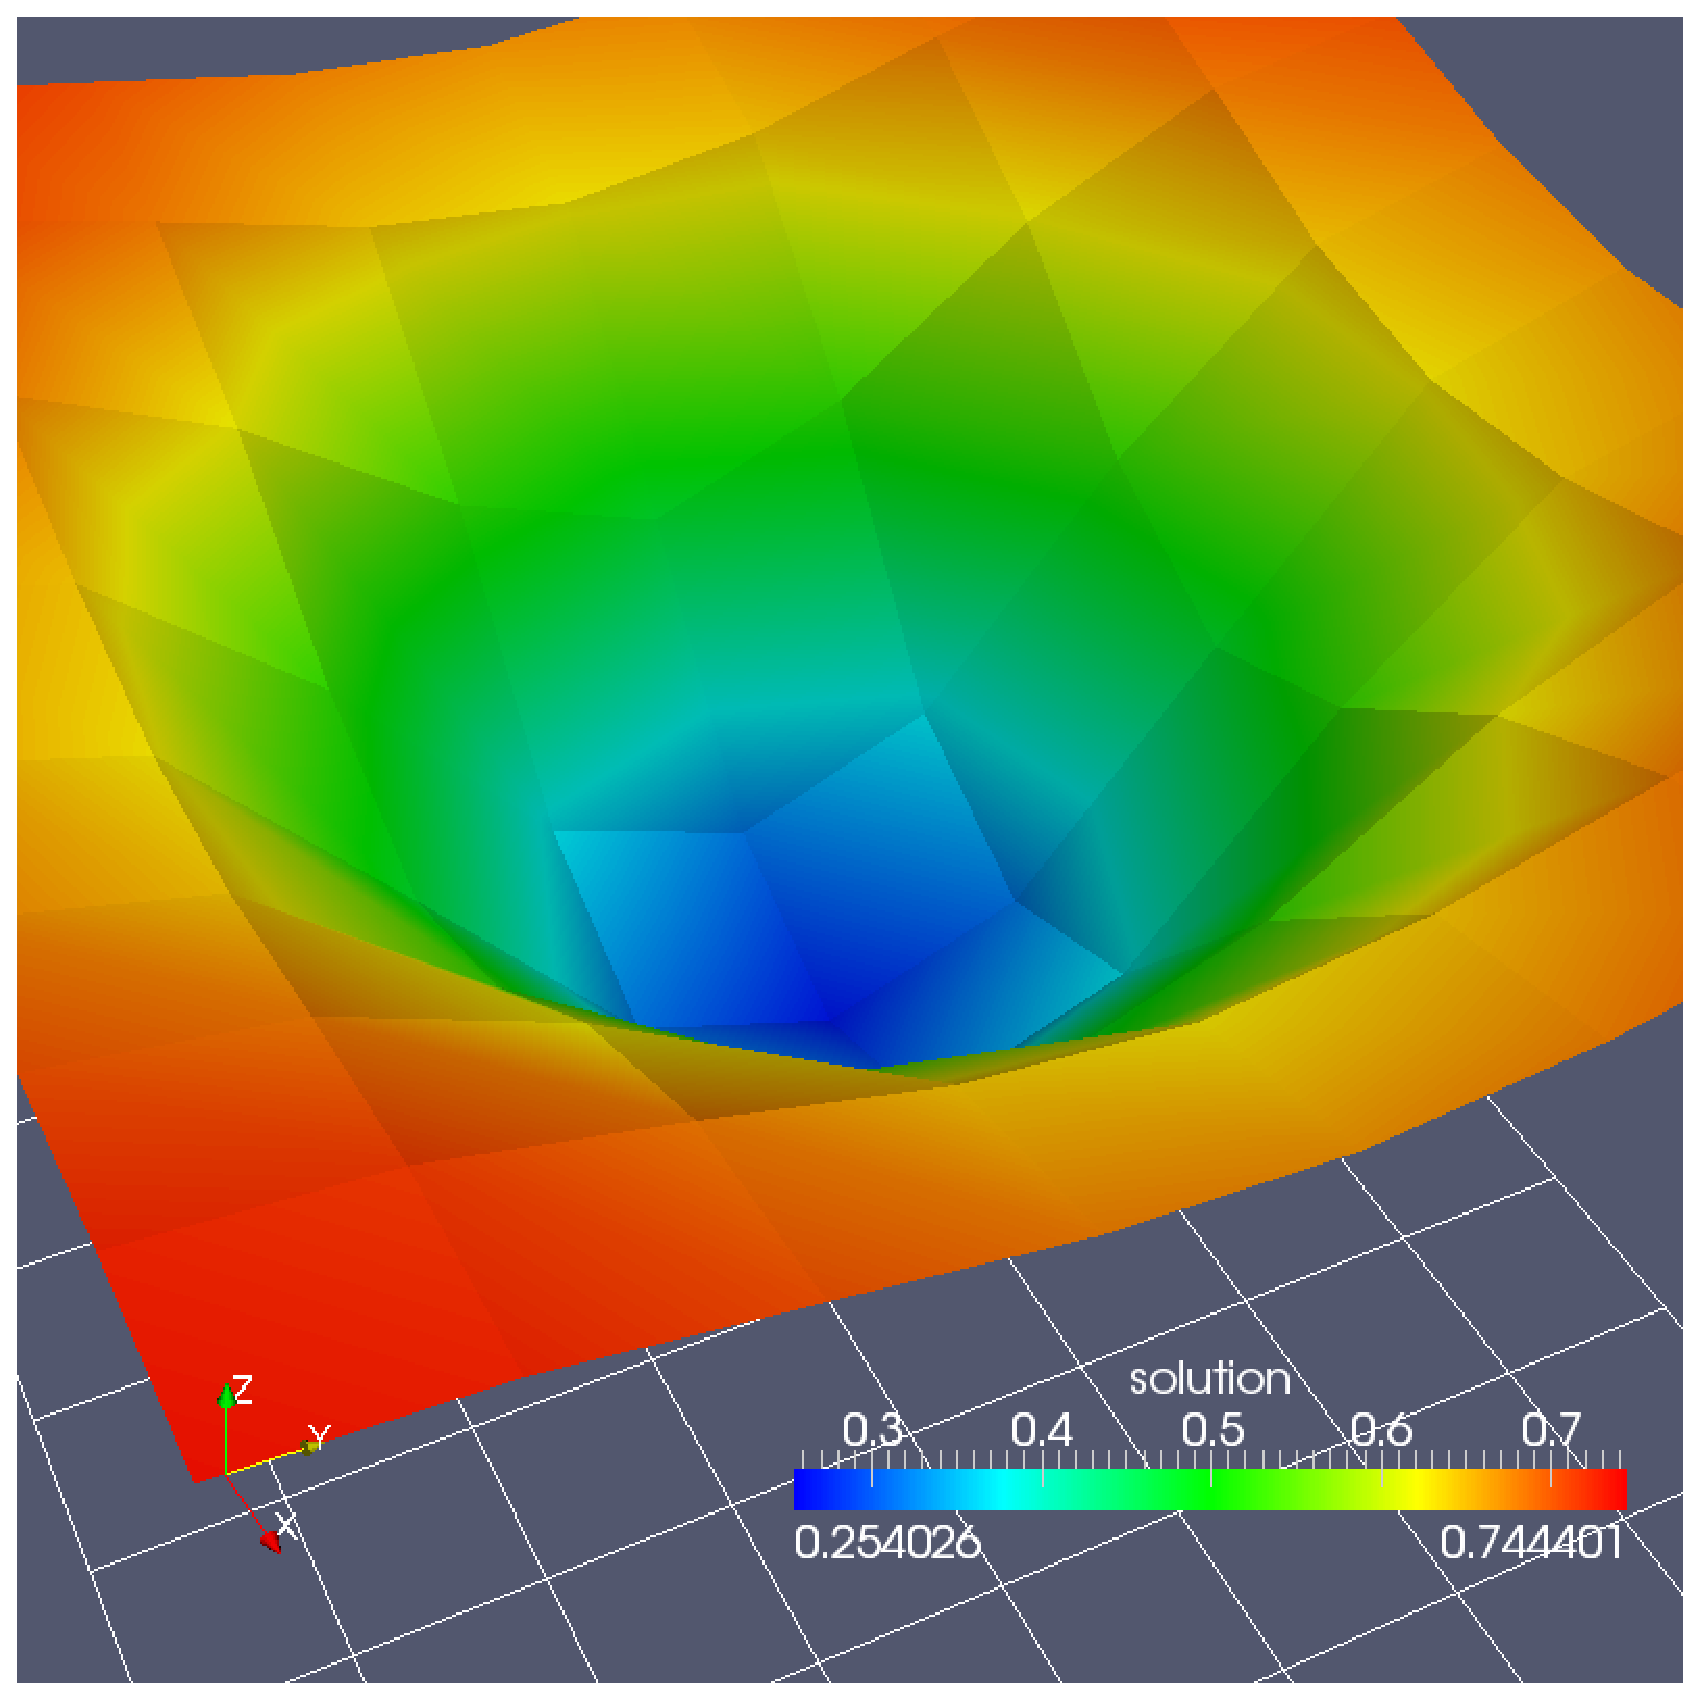
\includegraphics[width=0.32\textwidth]{./EPS/example01a_Q1} $\hspace{1mm}$
%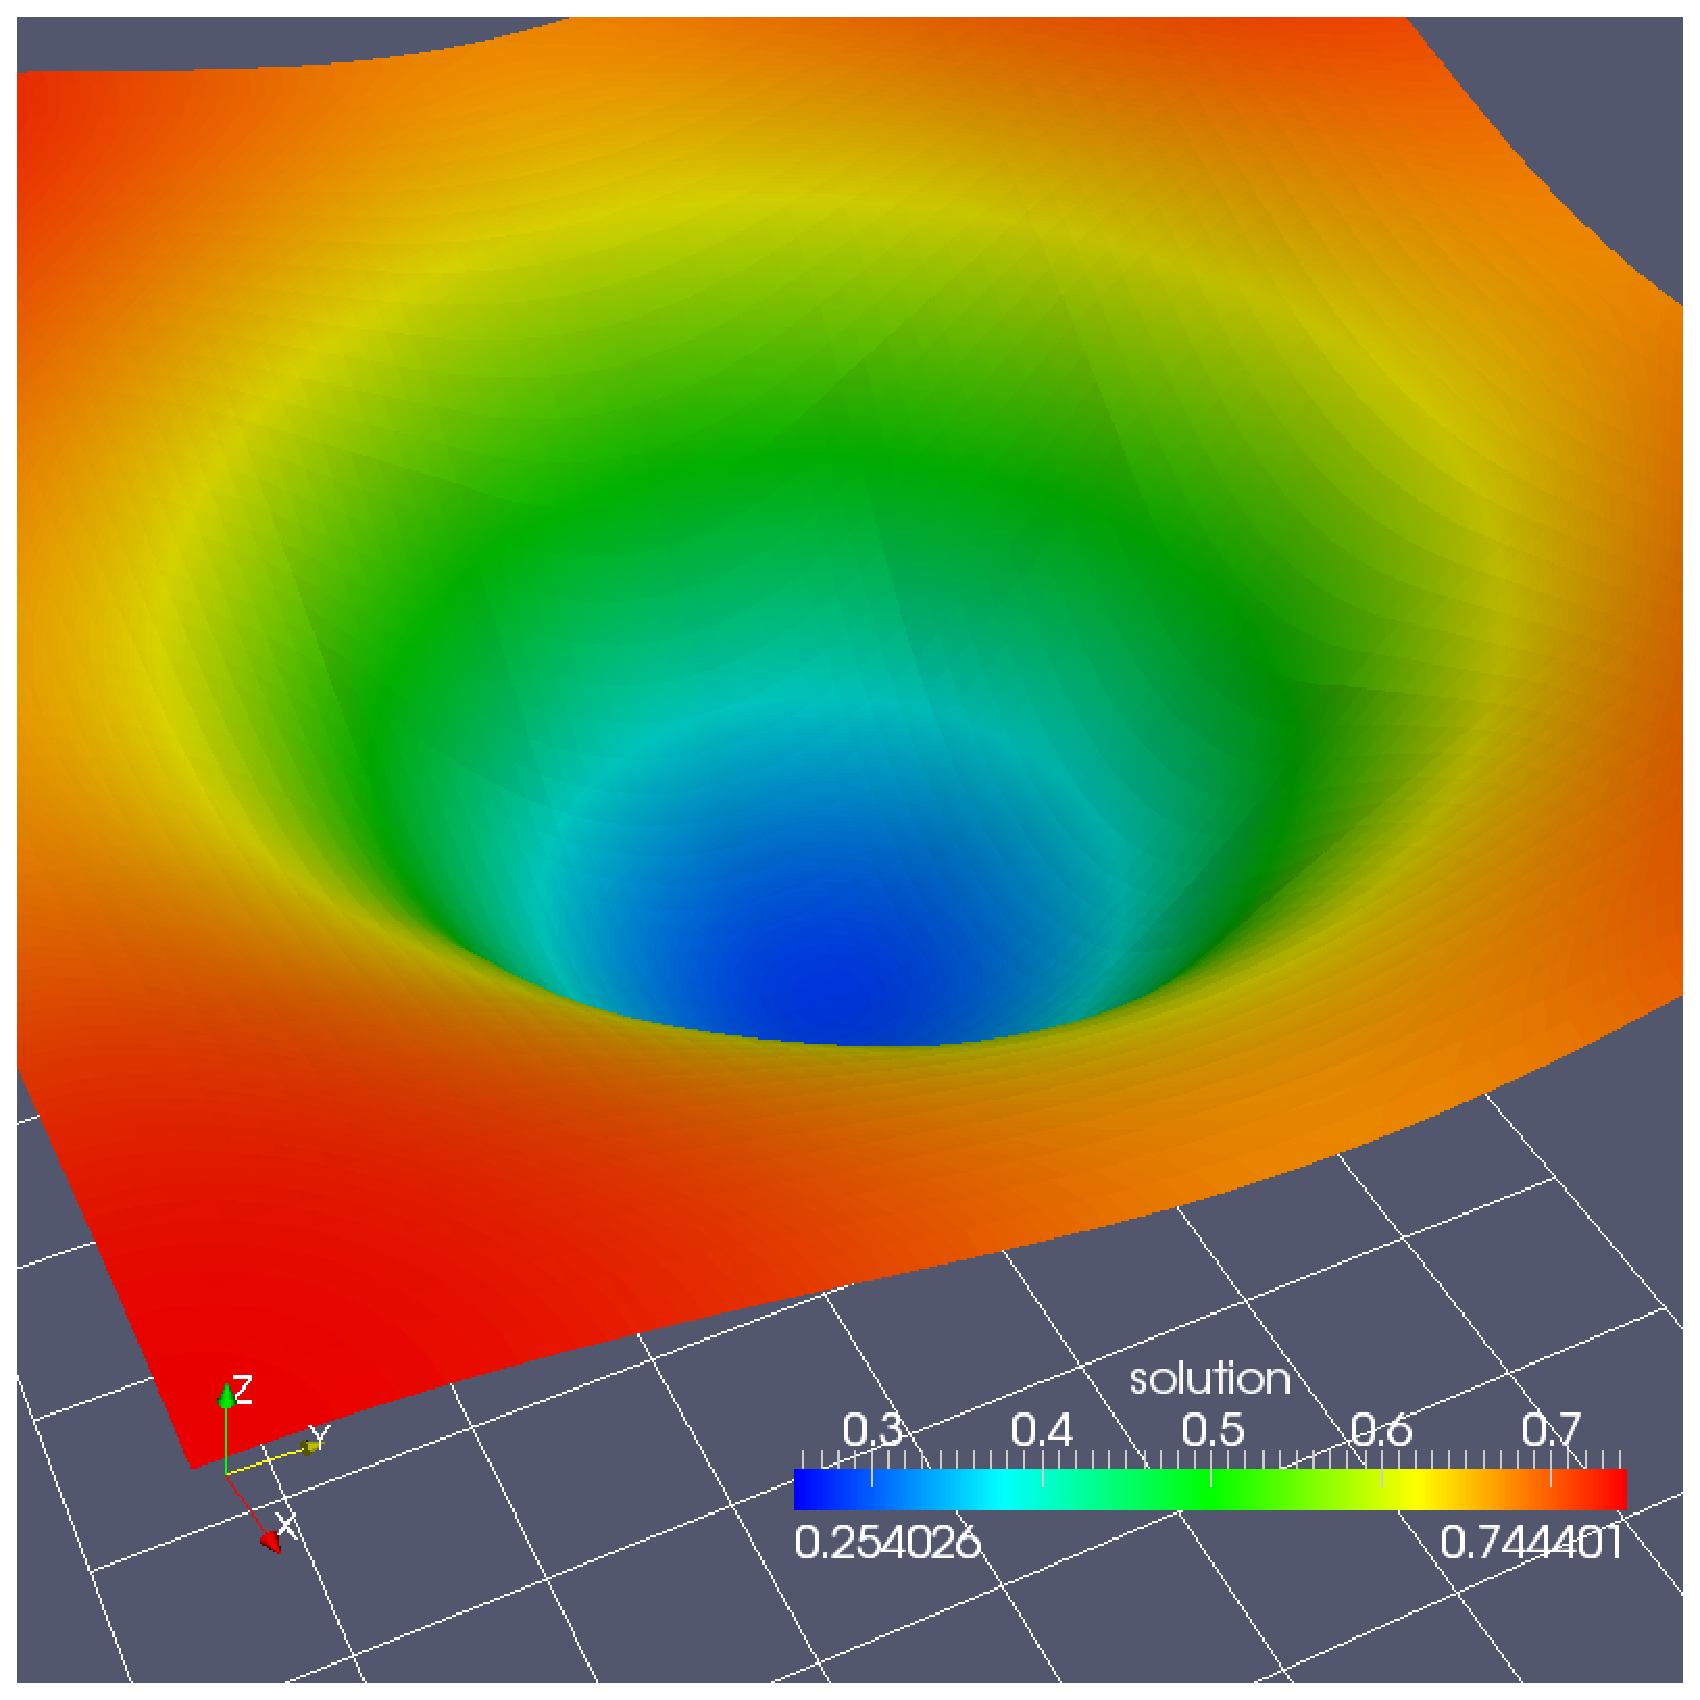
\includegraphics[width=0.32\textwidth]{./EPS/example01a_Q2} $\hspace{1mm}$
%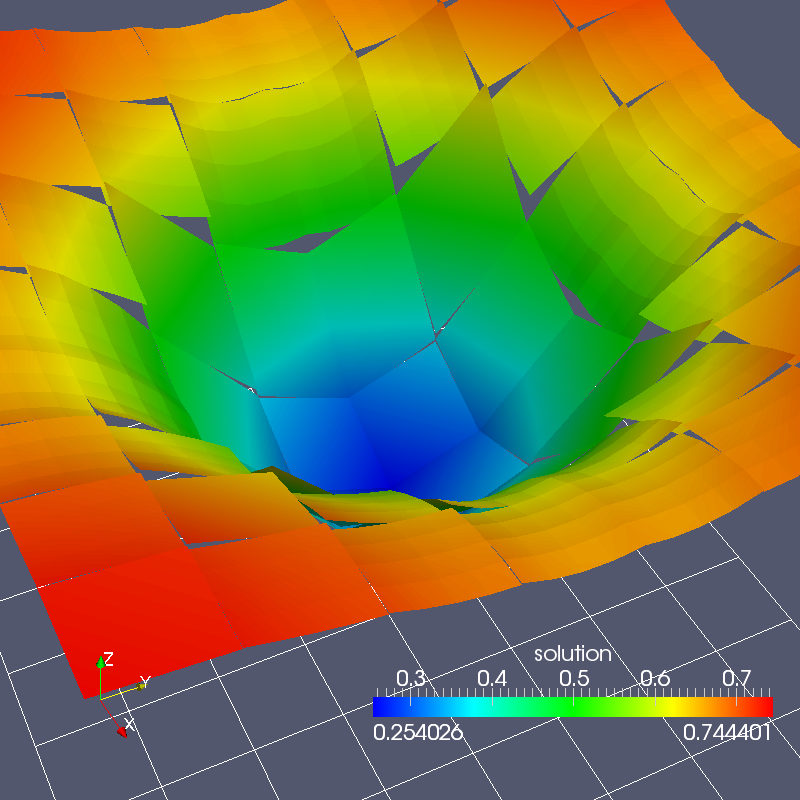
\includegraphics[width=0.32\textwidth]{./EPS/example01a_RT}
%
%$Q_1$ \hspace{30mm} $Q_2$ \hspace{30mm} $RT$
%\end{center}
%
%\mode<presentation>{
%More on that in the excercises!
%}
%\end{frame}
%
%\mode<article>{
%Figure \ref{fig:Example01aResults} shows visualizations of the results computed
%with \lstinline{example01}.
%\begin{figure}
%\begin{center}
%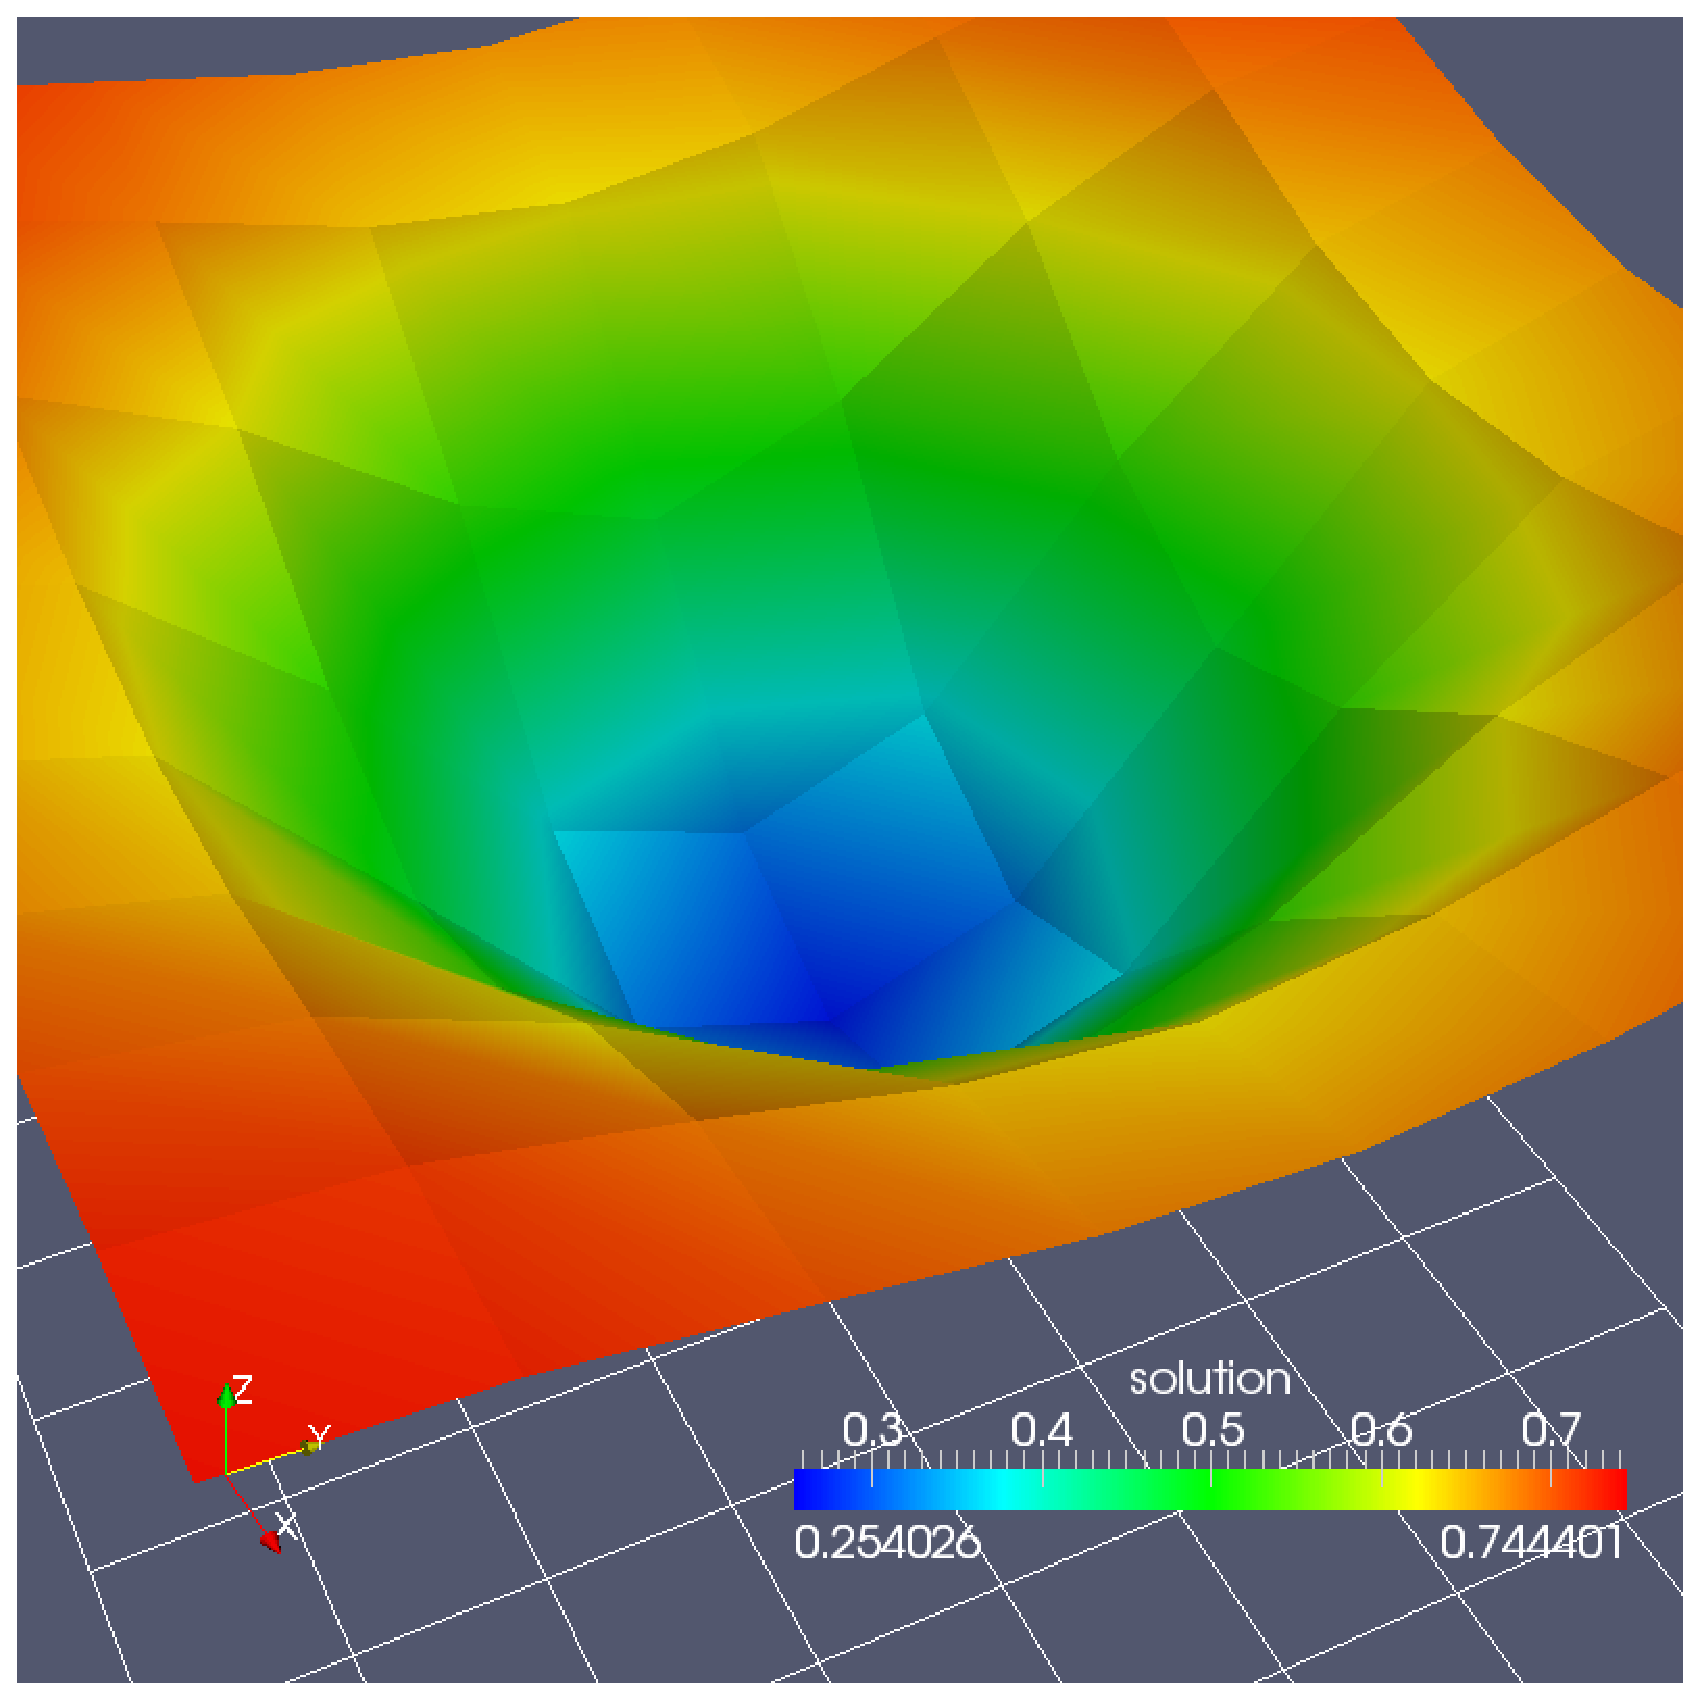
\includegraphics[width=0.32\textwidth]{./EPS/example01a_Q1} $\hspace{1mm}$
%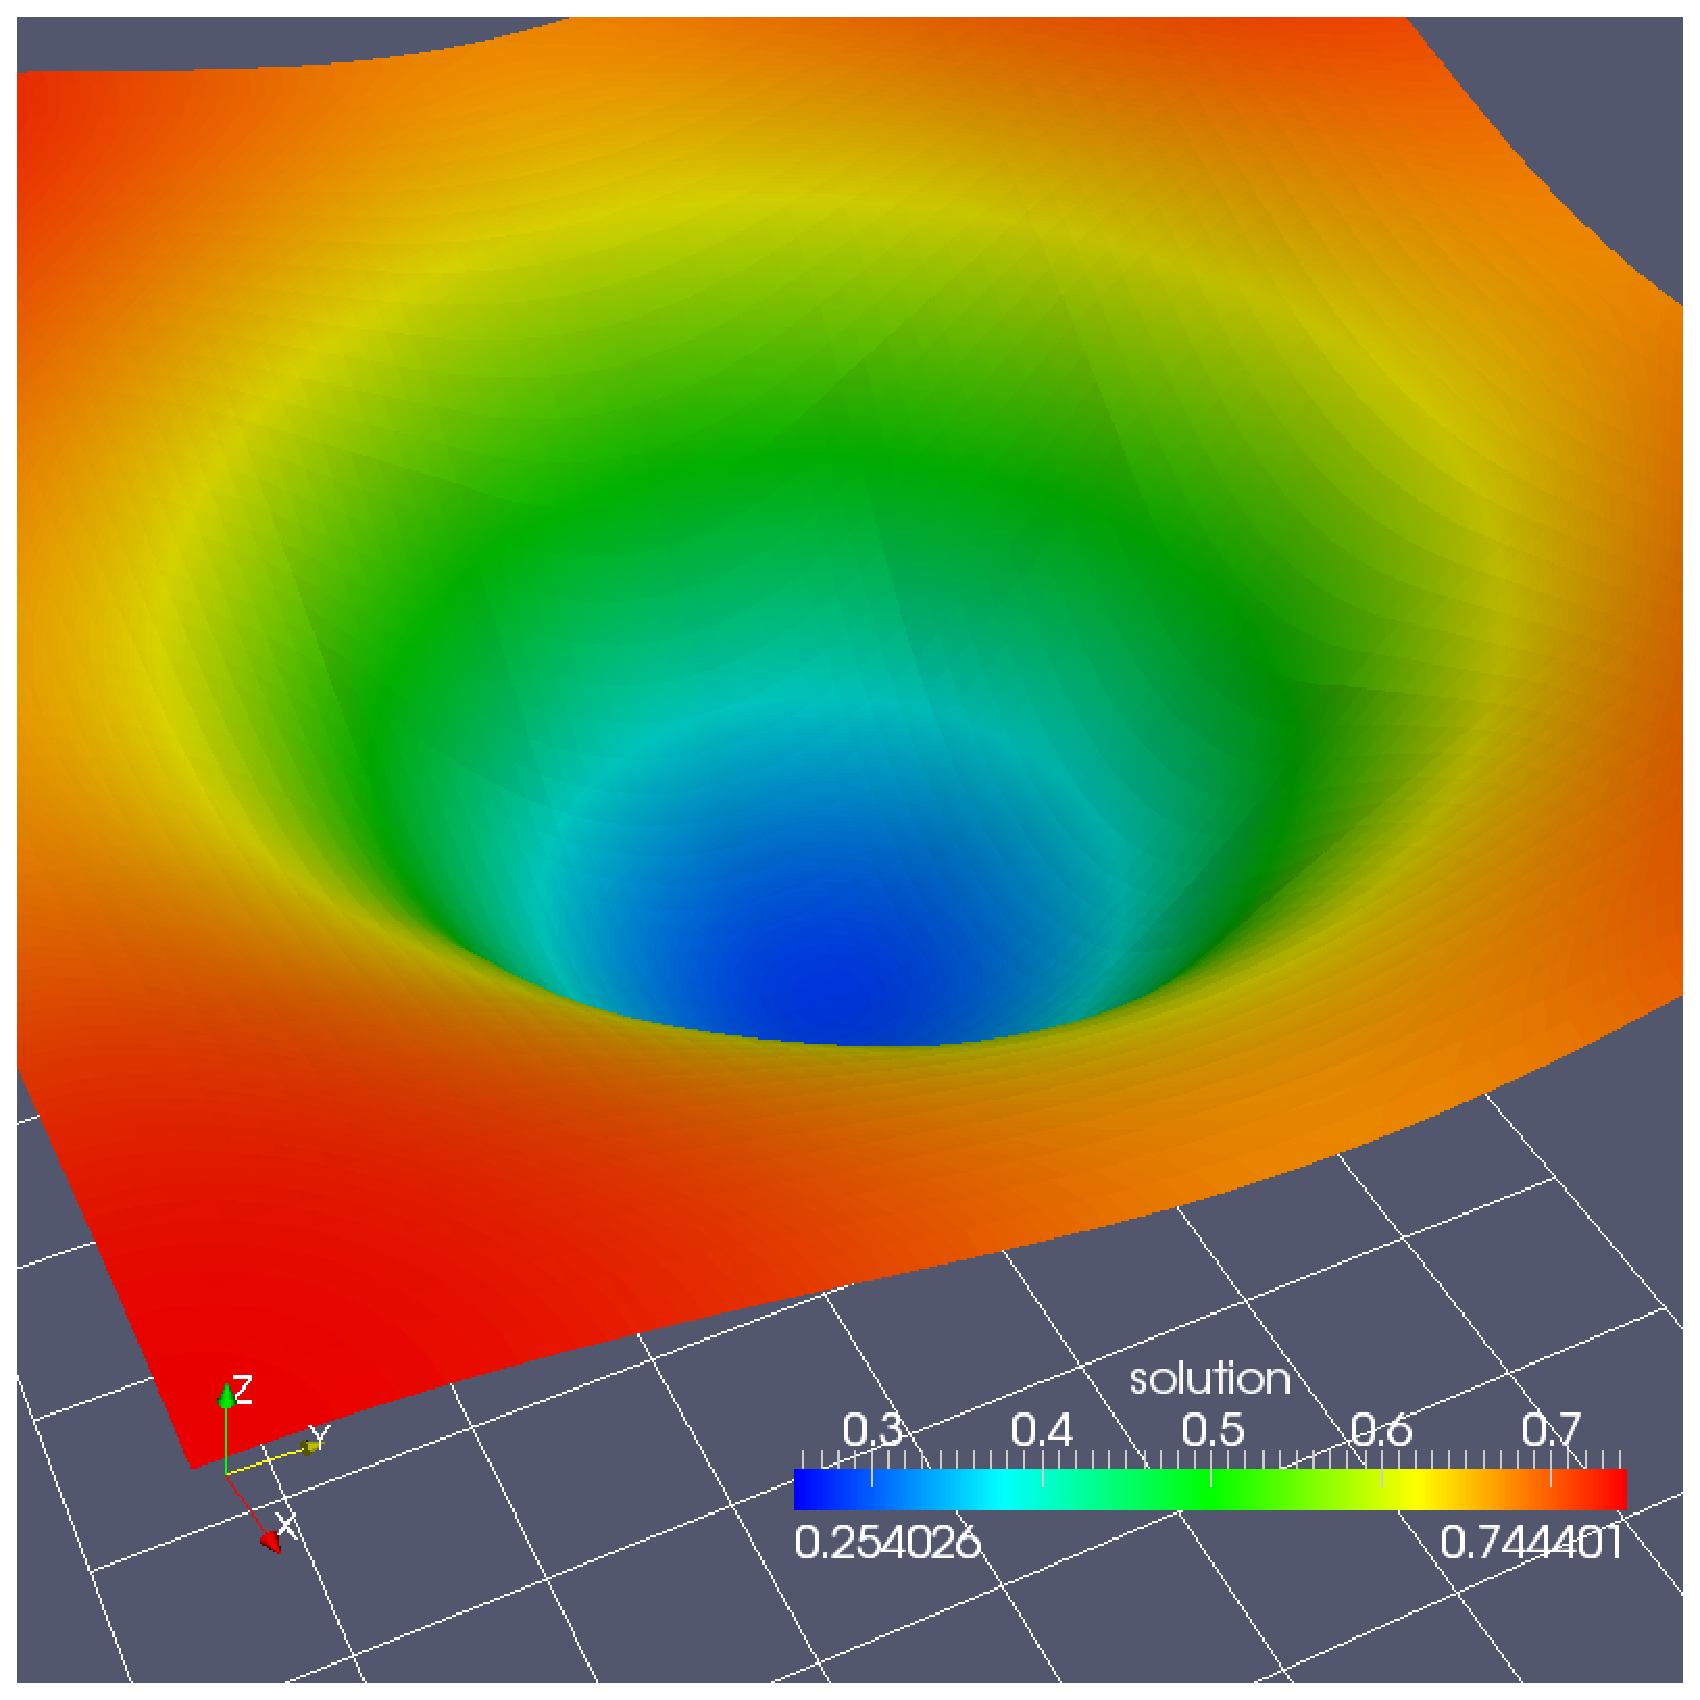
\includegraphics[width=0.32\textwidth]{./EPS/example01a_Q2} $\hspace{1mm}$
%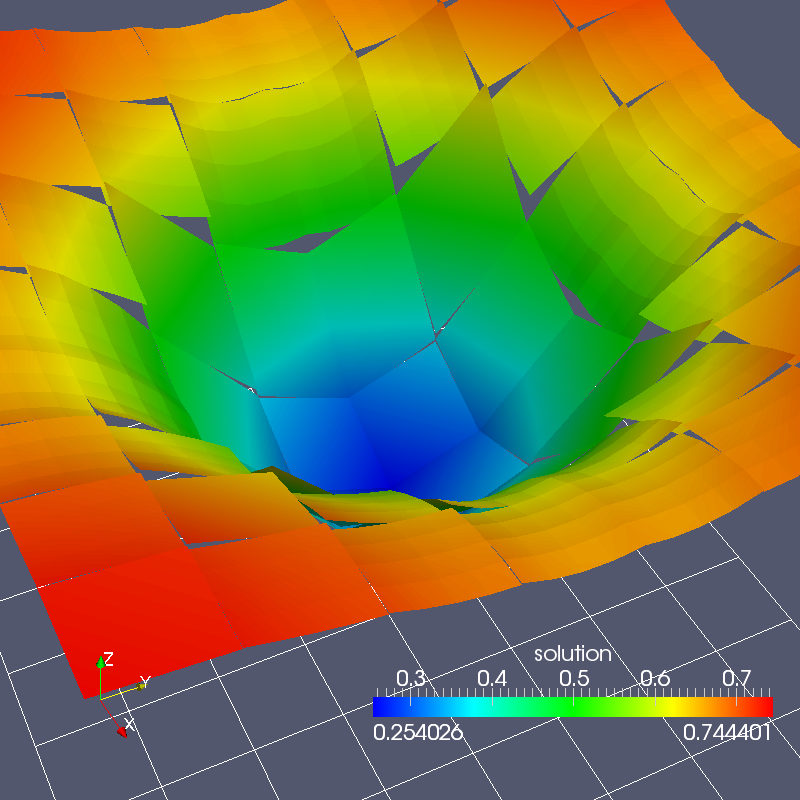
\includegraphics[width=0.32\textwidth]{./EPS/example01a_RT}
%\end{center}
%\caption{Results for example 1a computed with three different finite element spaces.
%From left: $Q_1$ elements, $Q_2$ elements, rotated bilinear (Rannacher-Turek)
%element on an $8 \times 8$ grid.}
%\label{fig:Example01aResults}
%\end{figure}
%}
%
%
%\begin{frame}
%\frametitle{Using $Q_2$ Elements}
%\ldots is quite simple, see \lstinline{example01a_Q2.hh}. Just
%\begin{itemize}
%\item Use another finite element map \lstinline{Q22DLocalFiniteElementMap}.
%\item Increase quadrature order on the local operator to 4.
%\item Use \lstinline{SubsamplingVTKWriter} to allow visualization of higher order polynomials.
%\item Use a new name for the output file.
%\end{itemize}
%
%Explore the Rannacher Turek element in \lstinline{example01a_RT.hh}
%\end{frame}
%
%
%\begin{frame}<presentation>[fragile,allowframebreaks,allowdisplaybreaks]
%\frametitle<presentation>{Unconstrained Elliptic Problem with $Q_2$}
%\framesubtitle<presentation>{File \texttt{examples/example01a\_Q2.hh}}
%\lstinputlisting[basicstyle=\tiny,numbers=left,
%numberstyle=\tiny, numbersep=2pt]{../../examples/example01a_Q2.hh}
%\end{frame}
%\mode<article>{
%\begin{Lst}[File examples/example01a\_Q2.hh] \mbox
%\nopagebreak
%\lstinputlisting[basicstyle=\scriptsize,numbers=left,
%numberstyle=\tiny, numbersep=2pt]{../../examples/example01a_Q2.hh}
%\end{Lst}}
%
%
%\begin{frame}
%\frametitle{Going Nonlinear}
%\ldots is also easy. Just
%\begin{itemize}
%\item Make a new local operator where the coefficients $a$ and $f$ depend on the solution $u$,
%see \lstinline{example01b_operator}.
%\item Use this new local operator in the grid operator space.
%\item Use class \lstinline{Newton} to solve the nonlinear algebraic problem.
%\item Use a new name for the output file :-).
%\end{itemize}
%\end{frame}
%
%\begin{frame}<presentation>[fragile,allowframebreaks,allowdisplaybreaks]
%\frametitle<presentation>{Unconstrained Nonlinear Elliptic Problem with $Q_2$}
%\framesubtitle<presentation>{File \texttt{examples/example01b\_Q2.hh}}
%\lstinputlisting[basicstyle=\tiny,numbers=left,
%numberstyle=\tiny, numbersep=2pt]{../../examples/example01b_Q2.hh}
%\end{frame}
%\mode<article>{
%\begin{Lst}[File examples/example01b\_Q2.hh] \mbox
%\nopagebreak
%\lstinputlisting[basicstyle=\scriptsize,numbers=left,
%numberstyle=\tiny, numbersep=2pt]{../../examples/example01b_Q2.hh}
%\end{Lst}}


\subsection{Importing and Meshing CAD-Geometries with Gmsh}
% CAD-Files
% Import
% Welcher Mesher?

\begin{frame}
  \frametitle{Common CAD-File formats}
  \begin{table}
    Amongst the most common CAD-File formats are
    \begin{center}
      \begin{tabular}{|c|c|c|}
        \hline
        Format & Ending & Description
        \\
        \hline
        STEP & \lstinline!.stp! &
        \\
        \hline
        BREP & \lstinline!.brp! &
        \\
        \hline
        IGES & \lstinline!.igs, .iges! &
        \\
        \hline
        GEO & \lstinline!.geo! & Native Gmsh format
        \\
        \hline
      \end{tabular}
      \caption{Some CAD file formats.}
      \label{tab:CADFileFormats}
    \end{center}
  \end{table}
\end{frame}

%\begin{frame}
%\frametitle{What is different ?}
%\begin{itemize}
%\item The residual form has a new term which is a boundary integral.
%\begin{itemize}
%\item There will be an additional method on the local operator.
%\end{itemize}
%\item The problem is solved in an affine subspace.
%We call $\tilde{U}$ a \textit{constrained space}.
%\item In the linear case it suffices to solve a problem with homogeneous Dirichlet
%boundary conditions:
%\begin{subequations}
%\begin{align*}
% -\Delta \bar{u} + a \bar{u}  &= f + \Delta w - a w &&\text{in $\Omega\subset\mathbb{R}^d$},\\
%                \bar{u} &= 0 &&\text{on $\Gamma_D\subseteq\partial\Omega$},\\
%-\nabla \bar{u} \cdot n &= j+\nabla w\cdot n &&\text{on $\Gamma_N=\partial\Omega\setminus\Gamma_D$},
%\end{align*}
%where $w$ is an extension of $g$ to $\Omega$ and $u = w + \bar{u}$.
%\end{subequations}
%\item In the nonlinear case this is not possible.
%\end{itemize}
%\end{frame}
%
%
%\begin{frame}
%\frametitle{Finite Element Spaces in Constrained Case}
%\begin{itemize}
%\item Define appropriate finite-dimensional subspace:
%\begin{equation*}
%\tilde{U}_h^k = \left \{ u \in U_h^k \,:\, u|_{\Gamma_D} = 0 \right\} \subset U_h^k.
%\end{equation*}
%(Mesh resolves the Dirichlet bopundary $\Gamma_D$.
%\item Provide extension $w\in U_h^k$ with ``$w=g$'' on $\Gamma_D$ in an appropriate sense.
%\item Obviously, $\text{dim}\tilde{U}_h^k < \text{dim} U_h^k$.
%\item Note: Dirichlet boundary conditions could also be handled by penalty methods.
%This can be done easily in PDELab but is not shown here.
%\end{itemize}
%\end{frame}
%
%\begin{frame}
%\frametitle{Realization of Dirichlet Constraints}
%\begin{itemize}
%\item Assume $\Phi_{U_h^k}$ is a Lagrange basis:
%\begin{equation*}
%\phi_j(x_i)=\delta_{i,j} \quad\text{where $x_i$ are the Lagrange points}.
%\end{equation*}
%\item Construct subspace via basis representation:
%\begin{itemize}
%\item $\mathcal{I}_{\tilde{U}_h^k} = \left\{ j\in \mathcal{I}_{U_h^k} \,:\,
%x_j \not\in \Gamma_D \right\} \subset \mathcal{I}_{U_h^k}$.
%\item $\Phi_{\tilde{U}_h^k} = \left\{ \phi_j\in \Phi_{U_h^k} \,:\,
%j \in \mathcal{I}_{\tilde{U}_h^k} \right\} \subset \Phi_{U_h^k}$.
%\item $\tilde{U}_h^k = \text{span}\Phi_{\tilde{U}_h^k}$.
%\end{itemize}
%\item For the coefficient space there are two options:
%\begin{enumerate}
%\item $\tilde{\mathbf{U}} = \mathbb{R}^{\mathcal{I}_{\tilde{U}_h^k}} \not\subseteq \mathbf{U}$.
%\item $\tilde{\mathbf{U}} = \left\{ \mathbf{u}\in\mathbf{U} \,:\, (\mathbf{u})_j = 0 \  \forall
%j \in \mathcal{I}_{U_h^k} \setminus \mathcal{I}_{\tilde{U}_h^k} \right\} \subset \mathbf{U}$.
%\end{enumerate}
%\item We choose (2) because
%\begin{itemize}
%\item $w + \tilde{u}$ is just adding coefficient vectors.
%\item Changing $\Gamma_D$, e.g. in time-dependent problems is easy.
%\end{itemize}
%\end{itemize}
%\end{frame}
%
%
%\begin{frame}
%\frametitle{General Constrained Spaces}
%\begin{itemize}
%\item Constrained spaces turn up in a number of other cases:
%\begin{itemize}
%\item Hanging nodes.
%\item Functions with zero average, rigid body modes.
%\item Varying polynomial degree in conforming finite elements ($p$-method).
%\item Periodic boundary conditions.
%\item Artificial essential boundary conditions or ghost degrees of freedom in parallelization.
%\end{itemize}
%\item PDELab has a general concept to handle all types of constraints.
%\item Given $U_h$ with index set $\mathcal{I}_{U_h^k}$, construct a basis of the subspace:
%\begin{itemize}
%\item Partition index set: $\mathcal{I}_{U_h^k} = \tilde{\mathcal{I}} \cup \bar{\mathcal{I}}$.
%\item Construct new basis from given basis:
%\begin{equation*}
%\tilde\phi_i = \phi_i + \sum\limits_{j\in\bar{\mathcal{I}}} \omega_{i,j} \phi_j, \qquad i\in\tilde{\mathcal{I}}.
%\end{equation*}
%\item $\tilde{U}_h$ is spanned by the new basis.
%\end{itemize}
%\item Constrained space defined by splitting $\tilde{\mathcal{I}} \cup \bar{\mathcal{I}}$
%and coefficients $\omega_{i,j}$.
%\end{itemize}
%\end{frame}


\subsection{Attaching Data to a CAD-Geometry and its Mesh}
% Gruppen in Gmsh
% Gmshreader nur eine Gruppe pro Element!
% PDELab-Code

%\begin{frame}
%\frametitle{Example 2 Overview}
%The first example implements model problem \eqref{Eq:Example01}.
%
%It consists of the following files:
%\begin{itemize}
%\item \lstinline{example02.cc} -- the file to be compiled, main function.
%\item \lstinline{example02_bctype.hh} -- a function giving the splitting $\partial\Omega = \Gamma_D \cup \Gamma_N$.
%\item \lstinline{example02_bcextension.hh} -- a function for $g$ and its extension $w$.
%\item \lstinline{example02_operator.hh} -- local operator including inhomogeneous Neumann boundary conditions.
%\item \lstinline{example02_Q1.hh} -- driver setting up and solving the problem.
%\end{itemize}
%\end{frame}
%
%\begin{frame}
%\frametitle{Driver for Solving Constrained Linear Problem}
%\framesubtitle{About \lstinline{example02_Q1.hh}}
%\begin{itemize}
%\item Class \lstinline{ConformingDirichletConstraints} parametrizes the grid function space
%with the possibility of having Dirichlet constraints.
%\item Function \lstinline{constraints} assembles constraints (i.e. the splitting
%$\mathcal{I}_{U_h^k} = \tilde{\mathcal{I}} \cup \bar{\mathcal{I}}$) from a given function.
%\item Function \lstinline{interpolate} initializes a coefficient vector from a given function.
%At the same time this defines the extension $w$ of $g$.
%\item The rest is the same as before.
%\end{itemize}
%\end{frame}
%
%\begin{frame}<presentation>[fragile,allowframebreaks,allowdisplaybreaks]
%\frametitle<presentation>{Constrained Elliptic Problem}
%\framesubtitle<presentation>{File \texttt{examples/example02\_Q1.hh}}
%\lstinputlisting[basicstyle=\tiny,numbers=left,
%numberstyle=\tiny, numbersep=2pt]{../../examples/example02_Q1.hh}
%\end{frame}
%\mode<article>{
%\begin{Lst}[File examples/example02\_Q1.hh] \mbox
%\nopagebreak
%\lstinputlisting[basicstyle=\scriptsize,numbers=left,
%numberstyle=\tiny, numbersep=2pt]{../../examples/example02_Q1.hh}
%\end{Lst}}
%
%\begin{frame}<presentation>[fragile,allowframebreaks,allowdisplaybreaks]
%\frametitle<presentation>{Boundary Condition Type Function}
%\framesubtitle<presentation>{File \texttt{examples/example02\_bctype.hh}}
%\lstinputlisting[basicstyle=\tiny,numbers=left,
%numberstyle=\tiny, numbersep=2pt]{../../examples/example02_bctype.hh}
%\end{frame}
%\mode<article>{
%\begin{Lst}[File examples/example02\_bctype.hh] \mbox
%\nopagebreak
%\lstinputlisting[basicstyle=\scriptsize,numbers=left,
%numberstyle=\tiny, numbersep=2pt]{../../examples/example02_bctype.hh}
%\end{Lst}}
%
%\begin{frame}<presentation>[fragile,allowframebreaks,allowdisplaybreaks]
%\frametitle<presentation>{Boundary Condition Extension Function}
%\framesubtitle<presentation>{File \texttt{examples/example02\_bcextension.hh}}
%\lstinputlisting[basicstyle=\tiny,numbers=left,
%numberstyle=\tiny, numbersep=2pt]{../../examples/example02_bcextension.hh}
%\end{frame}
%\mode<article>{
%\begin{Lst}[File examples/example02\_bcextension.hh] \mbox
%\nopagebreak
%\lstinputlisting[basicstyle=\scriptsize,numbers=left,
%numberstyle=\tiny, numbersep=2pt]{../../examples/example02_bcextension.hh}
%\end{Lst}}
%
%\begin{frame}[fragile]
%\frametitle{\lstinline{alpha_boundary} Method}
%Local operator is extended by a new method \lstinline{alpha_boundary}
%computing the boundary integral.
%
%\lstinline{alpha_boundary} has the following signature:
%\begin{lstlisting}[basicstyle=\scriptsize]
%template<typename IG, typename LFSU, typename X,
%         typename LFSV, typename R>
%void alpha_boundary (const IG& ig, const LFSU& lfsu_s, const X& x_s,
%                     const LFSV& lfsv_s, R& r_s) const
%\end{lstlisting}
%Where the arguments are:
%\begin{itemize}
%\item \lstinline{ig} -- intersection with domain boundary.
%\item \lstinline{lfsu_s} -- local basis $\hat\phi_{e,l}$ for trial space on inside element.
%\item \lstinline{x_s} -- local coefficients on inside element.
%\item \lstinline{lfsv_s} -- local basis $\hat\psi_{e,l}$ for test space on inside element.
%\item \lstinline{r_s} -- local contribution to residual on inside element.
%\end{itemize}
%\end{frame}
%
%
%\begin{frame}<presentation>[fragile,allowframebreaks,allowdisplaybreaks]
%\frametitle<presentation>{Local Operator with Neumann Boundary}
%\framesubtitle<presentation>{File \texttt{examples/example02\_operator.hh}}
%\lstinputlisting[basicstyle=\tiny,numbers=left,
%numberstyle=\tiny, numbersep=2pt]{../../examples/example02_operator.hh}
%\end{frame}
%\mode<article>{
%\begin{Lst}[File examples/example02\_operator.hh] \mbox
%\nopagebreak
%\lstinputlisting[basicstyle=\scriptsize,numbers=left,
%numberstyle=\tiny, numbersep=2pt]{../../examples/example02_operator.hh}
%\end{Lst}}
%
%\begin{frame}<presentation>
%\frametitle{Visualization of Constrained Problem Results}
%Neumann boundary condition at $x=1$, Dirichlet elsewhere.
%
%\begin{center}
%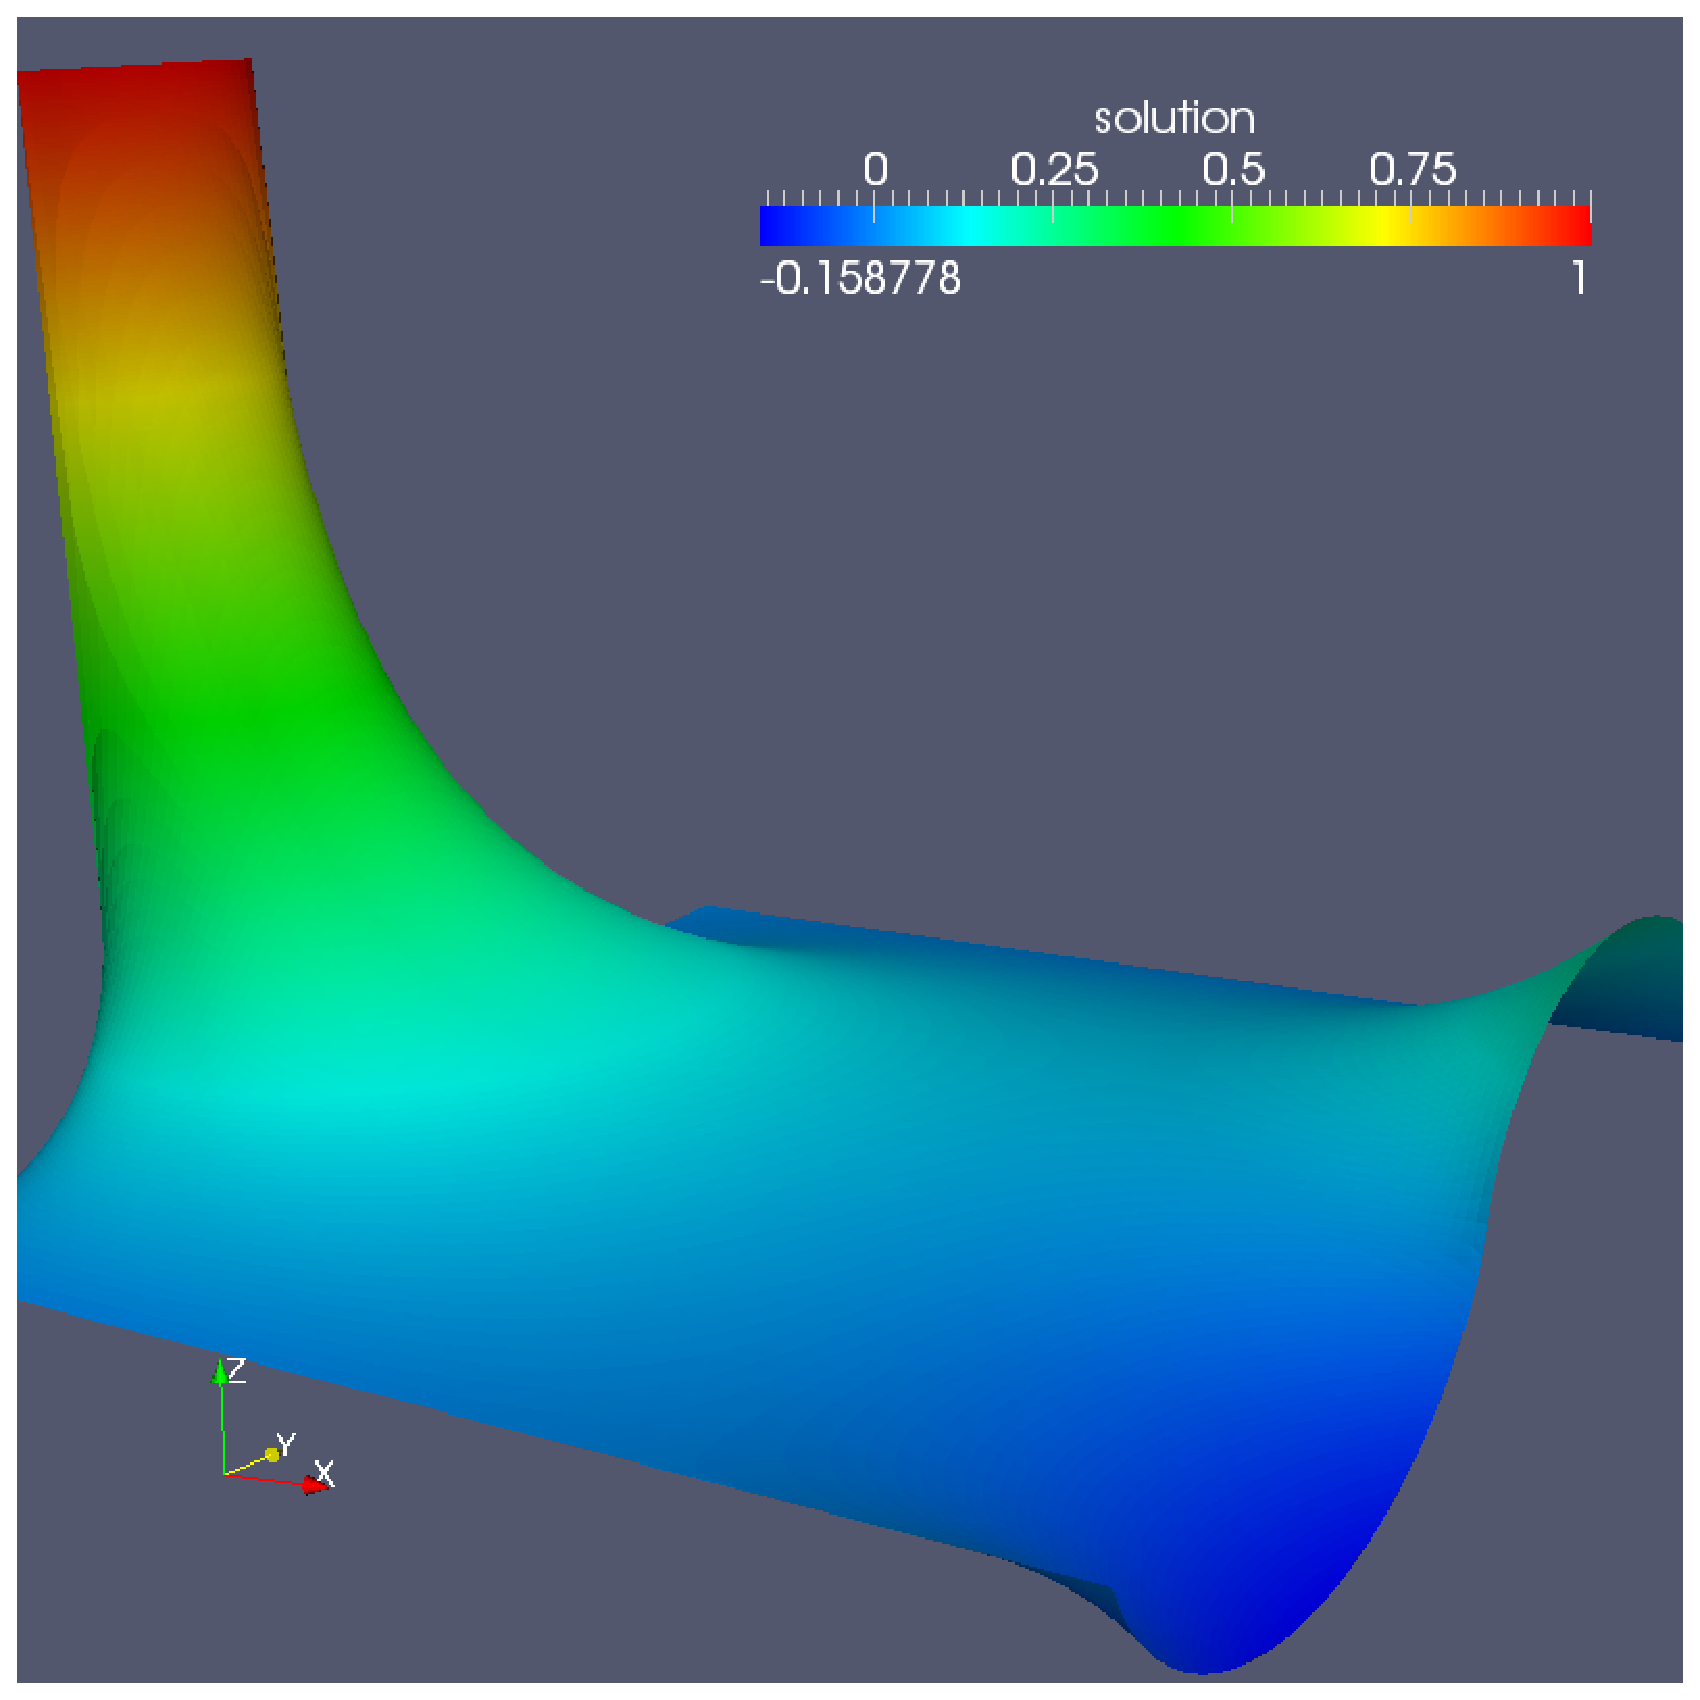
\includegraphics[width=0.48\textwidth]{./EPS/example02_Q1} \hspace{1mm}
%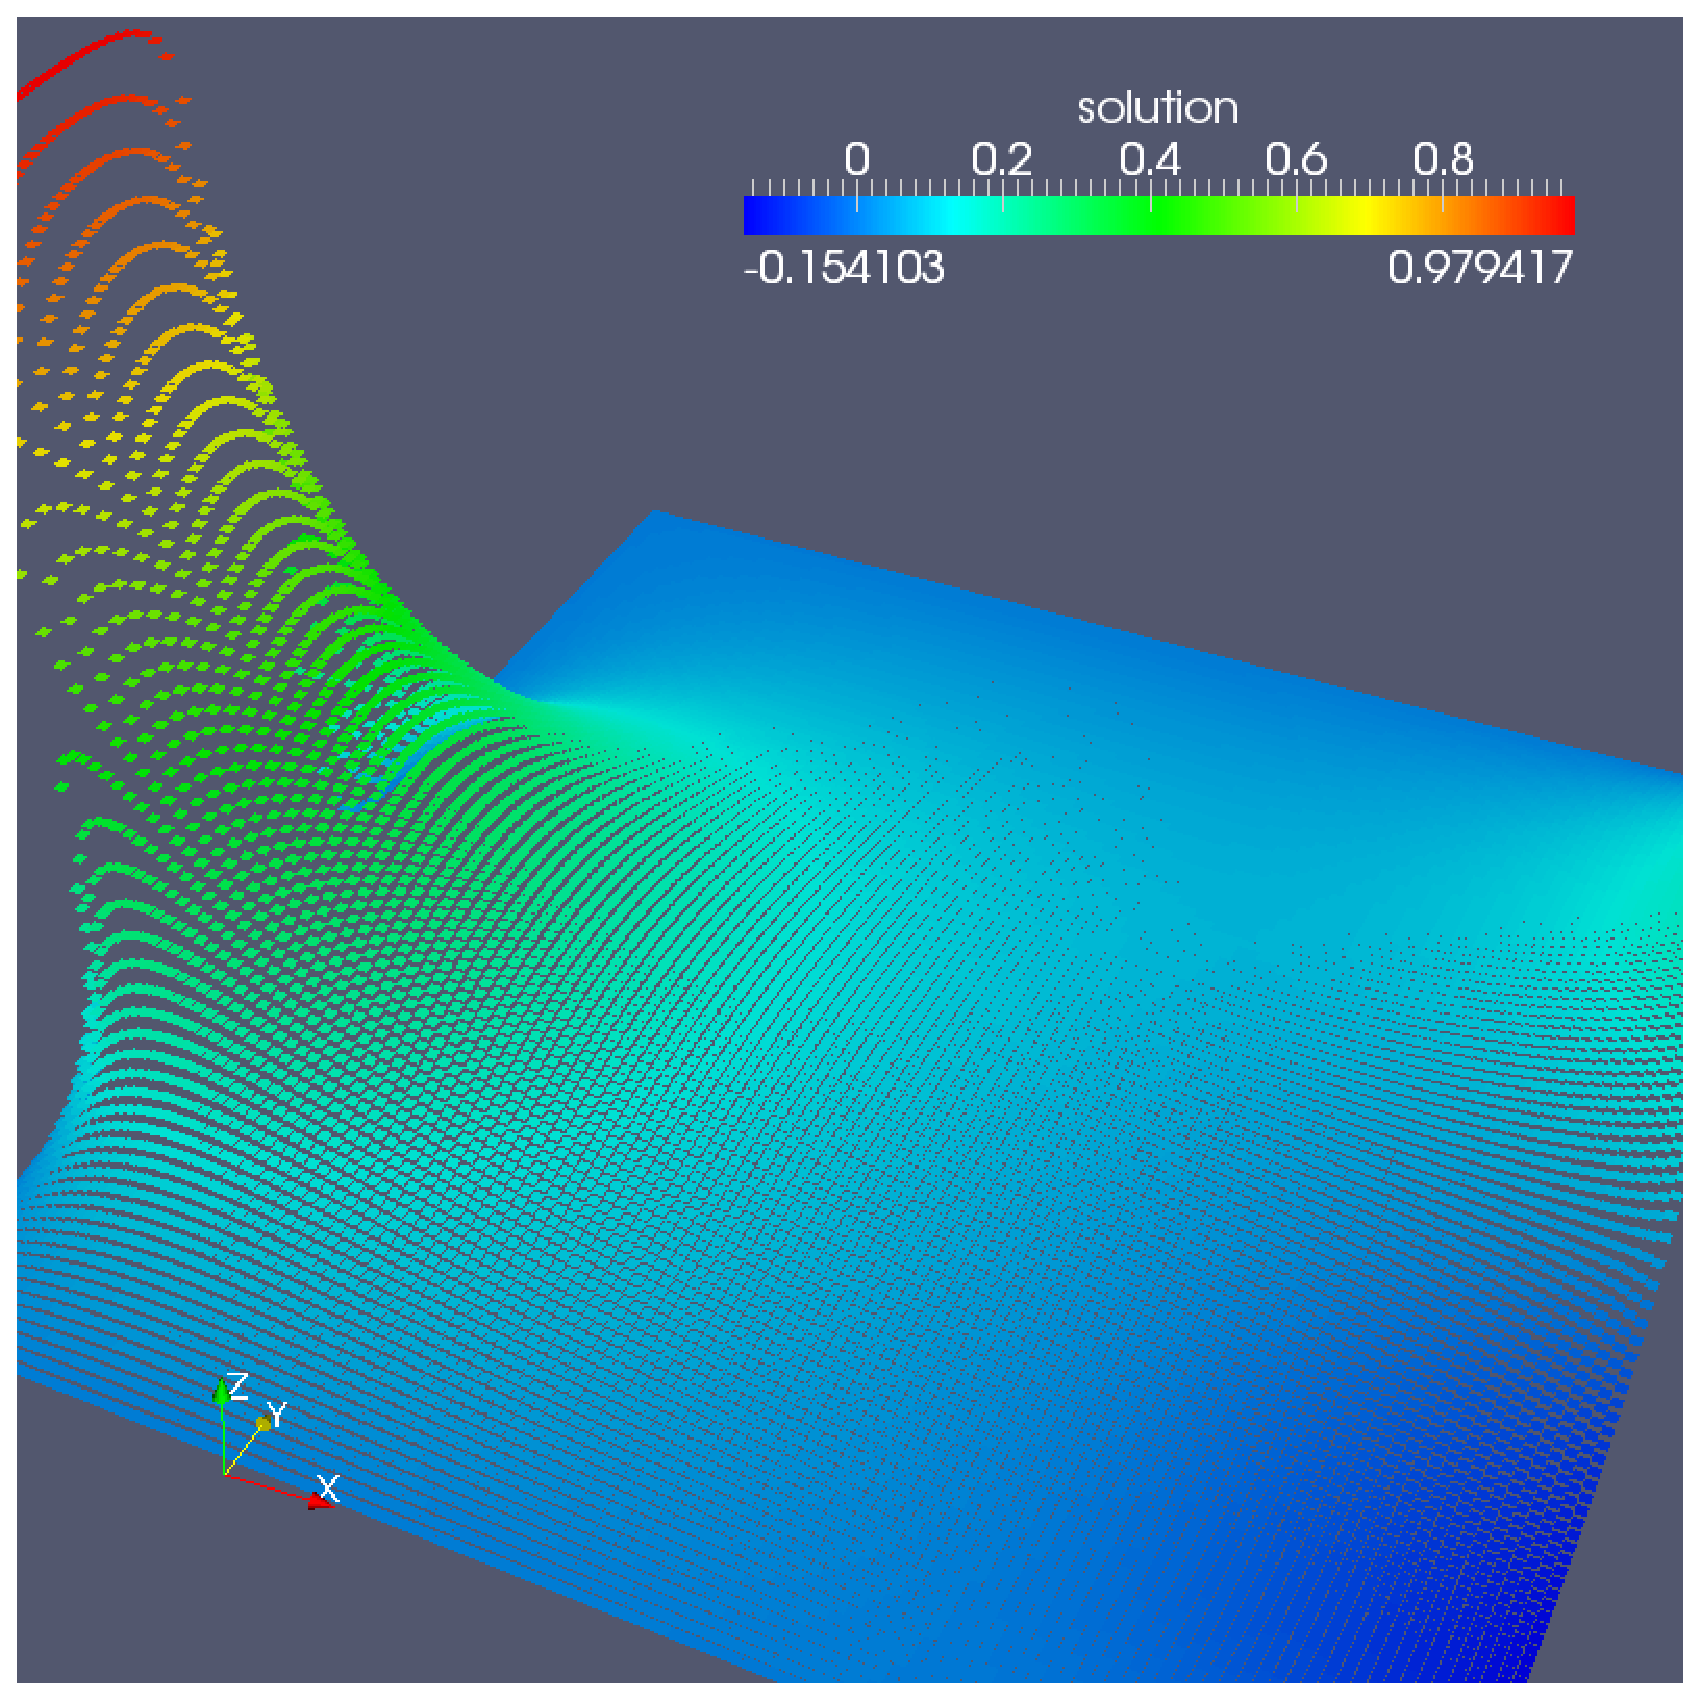
\includegraphics[width=0.48\textwidth]{./EPS/example04}
%\end{center}
%
%Conforming $Q_1$ from example 2 left and cell-centered finite volumes from example 4 right.
%\end{frame}
%
%\mode<article>{
%Figure \ref{fig:Example01aResults} shows visualizations of the results computed
%with \lstinline{example01}.
%\begin{figure}
%\begin{center}
%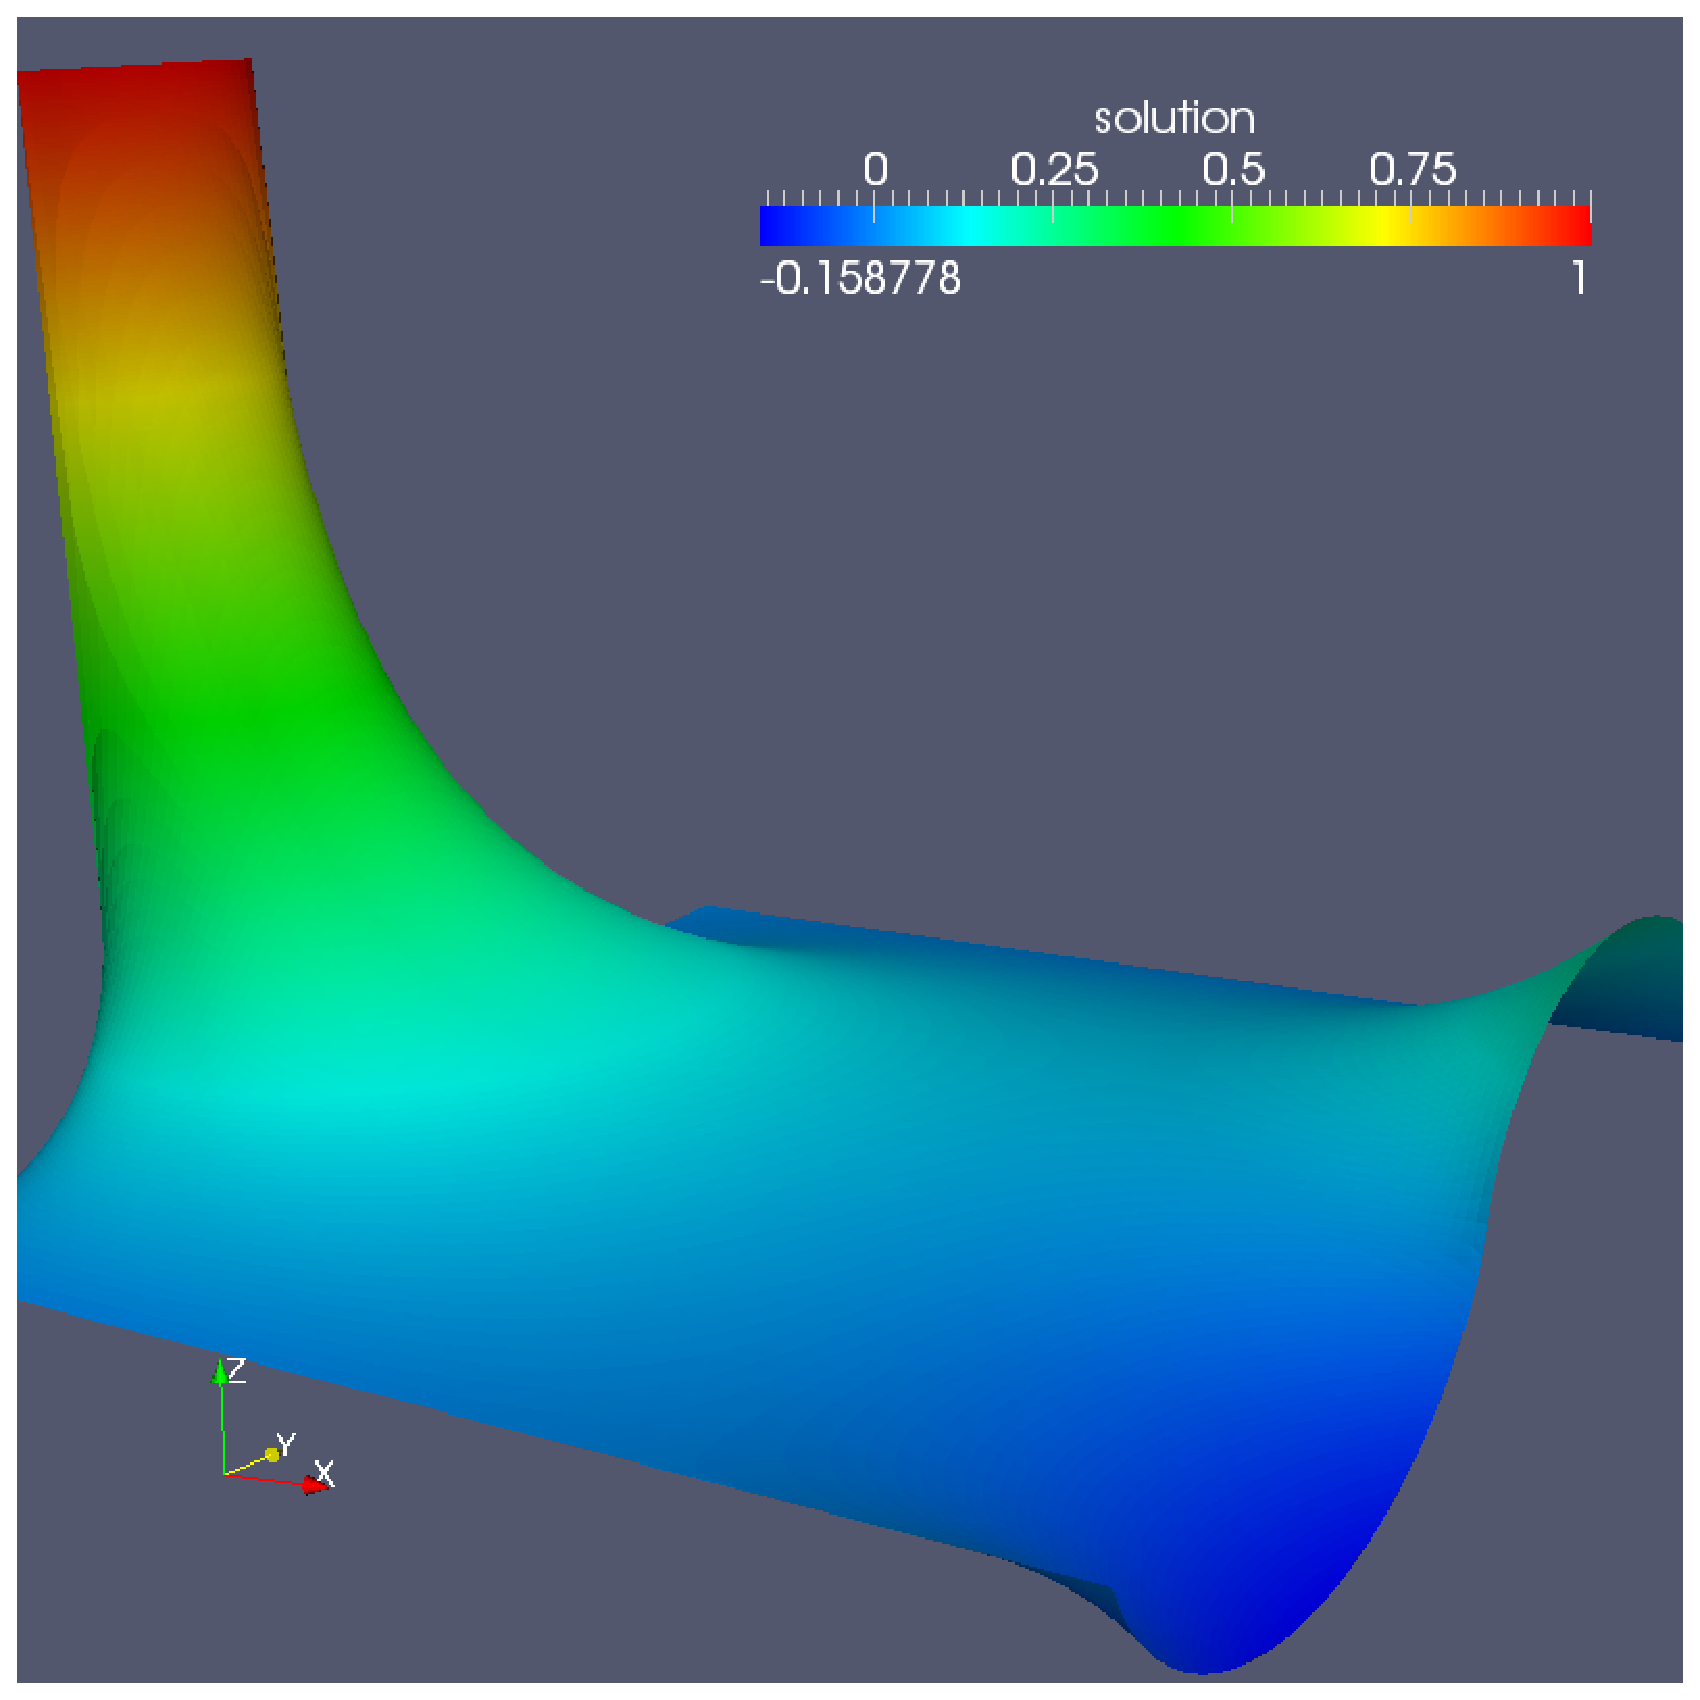
\includegraphics[width=0.48\textwidth]{./EPS/example02_Q1} \hspace{1mm}
%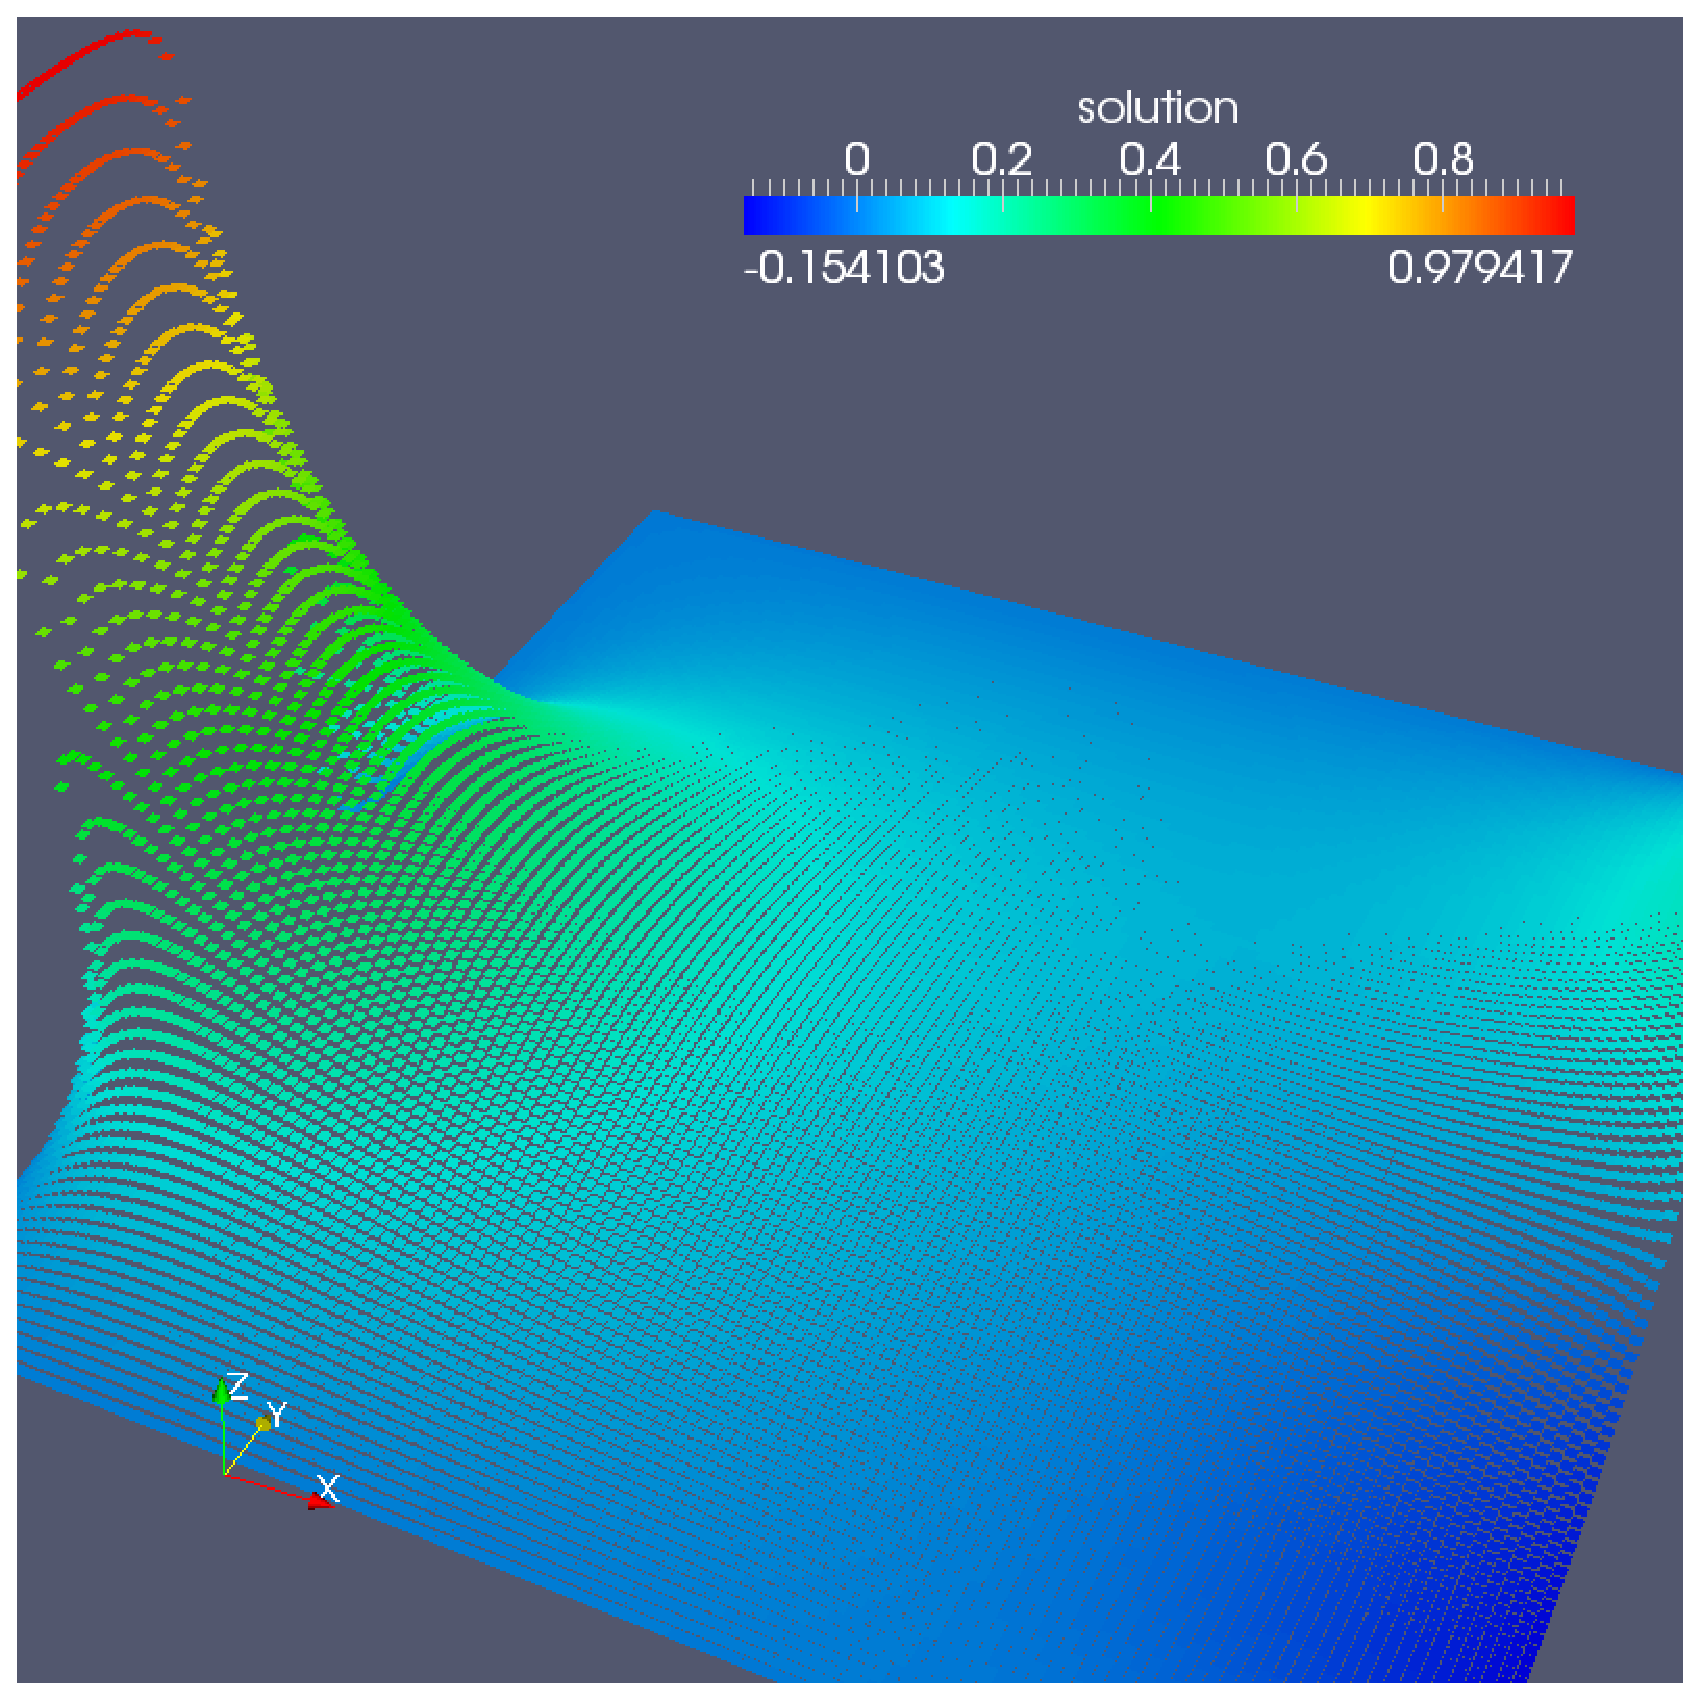
\includegraphics[width=0.48\textwidth]{./EPS/example04}
%\end{center}
%\caption{Result for example 2 computed with $Q_1$ elements on the right.
%Same problem solved with cell-centered finite volume method in example 4.}
%\label{fig:Example02Results}
%\end{figure}
%}
%
%\begin{frame}
%\frametitle{Remark on Local Operators}
%In practice one would access parameter functions such as $a, f, j$ and the boundary condition
%type from the implementation of the local operator.
%\end{frame}

\subsection{Salome}
% Gruppen in Gmsh
% Gmshreader nur eine Gruppe pro Element!
% PDELab-Code

\subsection{Other useful open source CAD-Tools}
% Gruppen in Gmsh
% Gmshreader nur eine Gruppe pro Element!
% PDELab-Code

\cleardoublepage
